\section{Konzept}

Dieses Kapitel beschreibt das Konzept, nach welchem das cloudbasierte Praxisrufsystem aus dem Vor-gängerprojekt erweitert wurde.
Die Konzepte wurden vor Beginn der Umsetzung definiert und während der Umsetzung laufend überarbeitet und erweitert.
Die folgende Dokumentation beschreiben die neuste Version des Konzepts und stellt damit das umgesetzte System dar.
Dabei wird nicht hervorgehoben, welche Teile zu Beginn definiert und welche Teile später überarbeitet oder ergänzt wurden.

Das Konzept gibt zuerst einen Überblick über das System als Ganzes.
Es werden die einzelnen Teile des Systems beschrieben und es werden Schritte definiert, um die Weiterentwicklung des Systems zu vereinfachen.
Anschliessend werden Konzepte für die Umsetzung der drei Features ''Native iOS Applikation'', ''Sprachsynthese'' und ''Gegensprechanlage'' beschrieben.


\subsection{Systemarchitektur}

Dieses Kapitel beschreibt die Komponenten des Praxisrufsystems und wie diese erweitert werden.
Das System wird um Komponenten zur Signalvermittlung und Sprachsynthese erweitert.
Weiter wird die interne Struktur des Cloudservices angepasst um die Weiterentwicklung und Betrieb des Systems zu vereinfachen.

\begin{figure}[h]
    \centering
    \begin{minipage}[b]{0.8\textwidth}
        \fbox{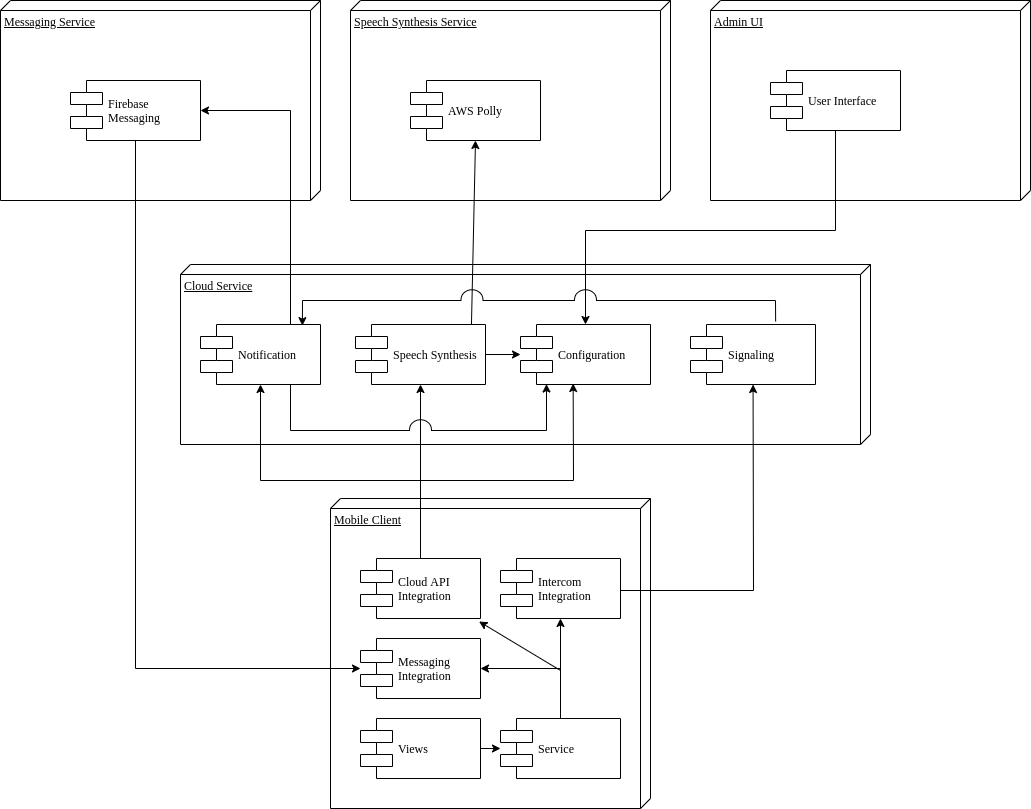
\includegraphics[width=\textwidth]{graphics/diagramms/Component_System_V03}}
        \caption{Systemkomponenten}
    \end{minipage}
\end{figure}

Abbildung 7.1 gibt einen Überblick über die Systemkomponenten und welche Teile diese beinhalten.
Die Pfeile zwischen Komponenten zeigen gerichtete Abfragen und damit eine Funktionale Abhängigkeit.
Alle dargestellten Komponenten sind entkoppelt und Abfragen finden nur über definierte Schnittstellen statt.

\subsubsection{Systemkomponenten}

Dieses Kapitel beschreibt die in Abbildung 7.1 abgebildeten Systemkomponenten.
Dabei wird für jede Komponente beschrieben, welche Aufgaben ihr zufallen und wie sie im Rahmen dieses Projektes erweitert wird.

\textbf{Cloudservice}

Der Cloudservice bildet das zentrale Serverkomponente des Praxisrufsystems.
Zu Beginn dieses Projektes umfasst der Cloudservice die beiden Domänen Notification und Configuration.
Dabei ist die Domäne Notification für das Versenden von Benachrichtigungen und die Domäne Configuration für die Verwaltung und Auswertung der Konfigurationen verantwortlich.
Die relevanten Empfänger für eine Benachrichtigung werden in der Configuration Domain ermittelt.
Um auf diese Informationen zugreifen zu können, muss aus der Notification Domain eine Abfrage an die Configuration Domain geschehen.
Die Configuration Domäne bietet dazu eine REST Schnittstelle~\cite{ip5}.

Die Trennung der Domänen wurde im Vorgängerprojekt lediglich auf Package-Ebene realisiert.
Mit diesem Projekt soll die Trennung einen Schritt weiter gehen.
Der Cloudservice wird Module aufgeteilt.
Diese Module werden weiterhin in einer einzelnen Applikation zusammengefasst.
Die Modularisierung können aber zu einem späteren Zeitpunkt in einzelne Microservices aufgeteilt werden.

Nachdem die Auftrennung in Module stattgefunden hat, wird der Cloudservice um die zwei Module Signaling und Speech Synthesis erweitert.
Das neue Modul Signaling ist für die Signalvermittlung zwischen Mobile Clients verantwortlich.
Es übernimmt die Aufgabe der Signaling Instanz für den Aufbau von Peer-To-Peer Sprachverbindungen mit WebRTC.
Das Modul Signaling hat eine gerichtete Abhängigkeit zum Module Notification.
Über das Notification Modul sollen Empfänger informiert werden, wenn ein Signal nicht zugestellt werden konnte.
Das neue Modul Speech Synthesis dient als Schnittstelle zu einem externen Provider für Sprachsynthese.
Dies ermöglicht es, die Sprachsynthese als Teil der API des Cloudservice anzubieten.
Dadurch können Clients aller Plattformen und auch Systeme, die künftig angebunden werden, auf die Sprachsynthese zugreifen.
Weil alle Clients die Daten aus derselben Schnittstelle beziehen, ist garantiert, dass die Konfiguration und Funktionsweise dieselbe für alle Clients ist. \\

\textbf{Mobile Client}

Der Mobile Client ist eine mobile Appliaktion, über welche das Praxisrufsystem bedient werden kann.
Der mit dem Vorgängerprojekt umgesetzte Mobile Client erlaubt es Benachrichtigungen zu versenden und empfangen~\cite{ip5}.
Dieser Mobile Client wird durch eine native iOS Applikation ersetzt.
Die native iOS App wird von Grund auf neu entwickelt.
Dabei muss sämtliche Funktionen des bestehenden Mobile Clients als Teil der nativen App neu implementiert werden.
Weiter werden die Funktionen Gegensprechanlage und Sprachsynthese für empfangene Benachrichtigungen umgesetzt.

\textbf{Admin UI}

Das Admin UI ist eine Webapplikation, über welche die Konfiguration des Praxisrufsystems verwaltet werden kann.
Die Konfiguration des Systems wird für Gegensprechanlage und Sprachsynthese erweitert.
Für die Gegensprechanlage müssen Buttons konfiguriert werden können.
Diese beinhalten Anzeigetext und Teilnehmer einer Sprachverbindung.
Weiter muss pro Benachrichtigung konfigurierbar sein, ob ihr Inhalt bei Empfang vorgelesen werden sollen.
Das Admin UI muss erweitert werden, um die Verwaltung der erweiterten Konfiguration zu ermöglichen.

\textbf{Messaging Service}

Der Messaging Service ist für die Zustellung von Push Benachrichtigungen an Mobile Clients verantwortlich.
Der Cloudservice muss an den Messaging Service angebunden sein, um Benachrichtigungen anhand der Konfiguration zu versenden~\cite{ip5}.
Die Anbindung des Cloudservices an den Messaging Service ist mit dem Vorgängerprojekt bereits umgesetzt und muss für dieses Projekt nicht angepasst werden.
Die neu entwickelte native iOS App muss hingegen an den Messaging Service angebunden werden, um Benachrichtigungen zu empfangen.
Als Messaging Service wird Firebase Cloud Messaging verwendet.

\textbf{Speech Synthesis Service}

Um Sprachsynthese zu ermöglichen, wird ein externer Service angebunden.
Dieser übernimmt die Konvertierung von Text aus Benachrichtigungen zu Sprachdaten.
Die Anbindung an den Speech Synthesis Service wird ausschliesslich im Cloudservice implementiert.
Sämtliche andere Komponenten die Sprachdaten benötigen, fragen diese beim Cloudservice ab.
Die REST API des Cloudservice wird um entsprechende Endpunkte erweitert.
Als Speech Synthesis Service wird Amazon Polly verwendet.

\subsubsection{Modularisierung Cloudservice}

Der mit dem Vorgängerprojekt umgesetzte Cloudservice ist als monolithische Applikation implementiert.
Er trennt intern die beiden Domänen Notification und Configuration.
Die Domäne Configuration ist für die Verwaltung und Auswertung der Konfiguration des Systems und die Domäne Notification für das Versenden von Benachrichtigungen verantwortlich.
Abhängigkeiten zwischen den beiden Domänen ist über eine REST-Schnittstelle abstrahiert.

Die Trennung der Domänen, erlaubt es die Anwendung zukünftig in mehrere Microservices aufzuteilen.
Diese könnten unabhängig betrieben und erweitert werden.
Weiter wird es dadurch möglich, einzelnen Teilen der Applikation mehr Ressourcen zuzuteilen.
Die Trennung der Domänen in eigene Microservices wurde noch nicht vorgenommen.
Die beiden Domänen wurden lediglich durch die Package Struktur innerhalb eines einzelnen monolithischen Services getrennt.

Die Trennung der Domänen innerhalb des Cloudservice wird weiter verstärkt.
Teile der Applikation werden neu in Module aufgeteilt.
Dabei wird pro Domäne ein Modul erstellt.
Dieses kapselt sämtliche Domänenobjekte, Services und Schnittstellen der jeweiligen Domäne.
Dadurch ist garantiert, dass die Domänen sauber voneinander getrennt sind.
Sämtliche Kommunikation zwischen den Modulen muss über REST-Schnittstellen geschehen.

Es werden die vier Domänen-Module Configuration, Notification, Spech Synthesis und Signaling definiert.
Das Modul Configuration beinhaltet alle Domänenobjekte, Services und Schnittstellen für die Verwaltung, Auswertung und Abfrage der Systemkonfiguration.
Das Modul Notification beinhaltet alle Domänenobjekte, Services und Schnittstellen für das Versenden von Benachrichtiungen.
Das Modul Speech Synthesis beinhaltet die Anbindung an den Speech Synthesis Service und stellt eine Schnittstelle zur verfügung über den das restliche System Sprachdaten beziehen kann.
Das Modul Signaling beinhaltet Domänenobjekte, Services und Schnittstellen für die Signalvermittlung zwischen Mobile Clients.

Weiter werden die zwei Module Commons und App definiert.
Komponenten, welche in mehr als einer Domäne verwendet werden, werden in ein zusätzliches Commons Modul verlegt.
Dazu gehören Data Transfer Objects für Schnittstellen zwischen den Modulen, geteilte Clients um Abfragen auf andere Module abzusetzen sowie Komponenten für Security und Fehlerhandling.
Neben den Modulen App und Commons, werden vier weitere Module für die Domänen Configuration, Notification, Speech Synthesis und Signaling erstellt.

Der Cloudservice wird weiterhin als monolithische Applikation betrieben.
Die Modularisierung garantiert dabei eine strikte Trennung der Domänen.
In Zukunft können einzelne Module aus dem Cloudservice ausgelöst und als eigenständige Applikationen betrieben werden.

\clearpage

\subsubsection{Domänenmodell Cloudservice}

Das Domänenmodell Cloudservices wird für die Integration von Sprachsynthese und Gegensprechanlage erweitert.
Abbildung 7.2 gibt eine Übersicht über das vollständige Domänenmodell der Domänen Configuration und Notification.
Die neuen Domänen Speech Synthesis und Signaling führen keine persistierten Daten.
Die Services und Komponenten dieser Domänen sind in den Kapiteln 7.3 und 7.4 beschrieben.

\begin{figure}[h]
    \centering
    \begin{minipage}[b]{0.9\textwidth}
        \fbox{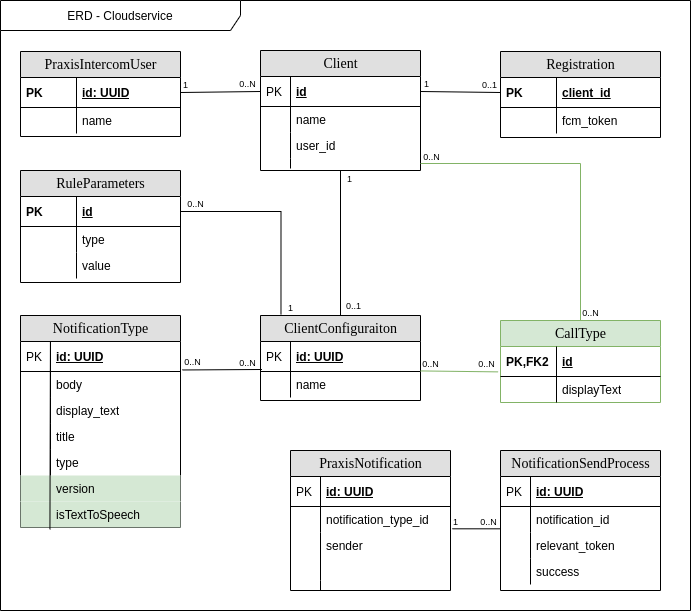
\includegraphics[width=\textwidth]{graphics/diagramms/erd_v02}}
        \caption{Entitiy Relation Diagramm - Cloudservice}
    \end{minipage}
\end{figure}

\clearpage

\subsection{Native iOS Applikation}

Dieses Kapitel beschreibt das Konzept für einen nativen iOS Client zur Bedienung von Praxisruf.
Es wird Entwurf und Funktionsweise der notwendigen Ansichten der Benutzeroberfläche beschrieben.
Weiter wird definiert, wie die aus dem Vorgängerprojekt zu migrierenden Funktionen in eine native iOS Applikation integriert werden können.
Dies beinhaltet insbesondere Anbindung der API des Cloudservice und Firebase Cloud Messaging.
Die Integration von Gegensprechanlage und Sprachsynthese wird nur im Rahmen des Entwurfs der Benutzeroberfläche beschrieben.
Eine detaillierte Beschreibung der Konzepte für diese Features folgt in den Kapiteln 7.3 und 7.4.


\subsubsection{Benutzeroberfläche}

Die Ansichten zur Anmeldung und Zimmerauswahl werden analog zum bestehenden Mobile Client umgesetzt.
Die Loginseite beinhaltet einen kurzen Willkommenstext und ein Logo für Praxisruf.
Darunter findet sich ein einfaches Formular zur Eingabe von Benutzername und Passwort, sowie ein Button zur Bestätigung.

\begin{figure}[h]
    \centering
    \begin{minipage}[b]{0.4\textwidth}
        \fbox{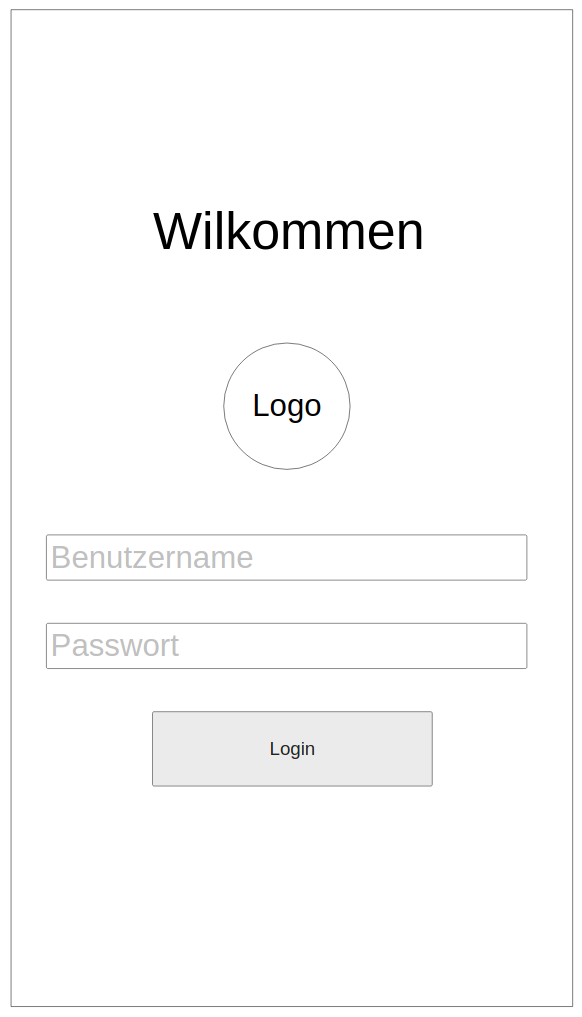
\includegraphics[width=\textwidth]{/home/joshua/FHNW/dev/IP6/IP6_Bachelorarbeit_Bericht_Cloudbasiertes_Praxisrufsystem/src/graphics/mockups/mockup_login}}
        \caption{Mockup Login}
    \end{minipage}
    \hfill
    \begin{minipage}[b]{0.4\textwidth}
        \fbox{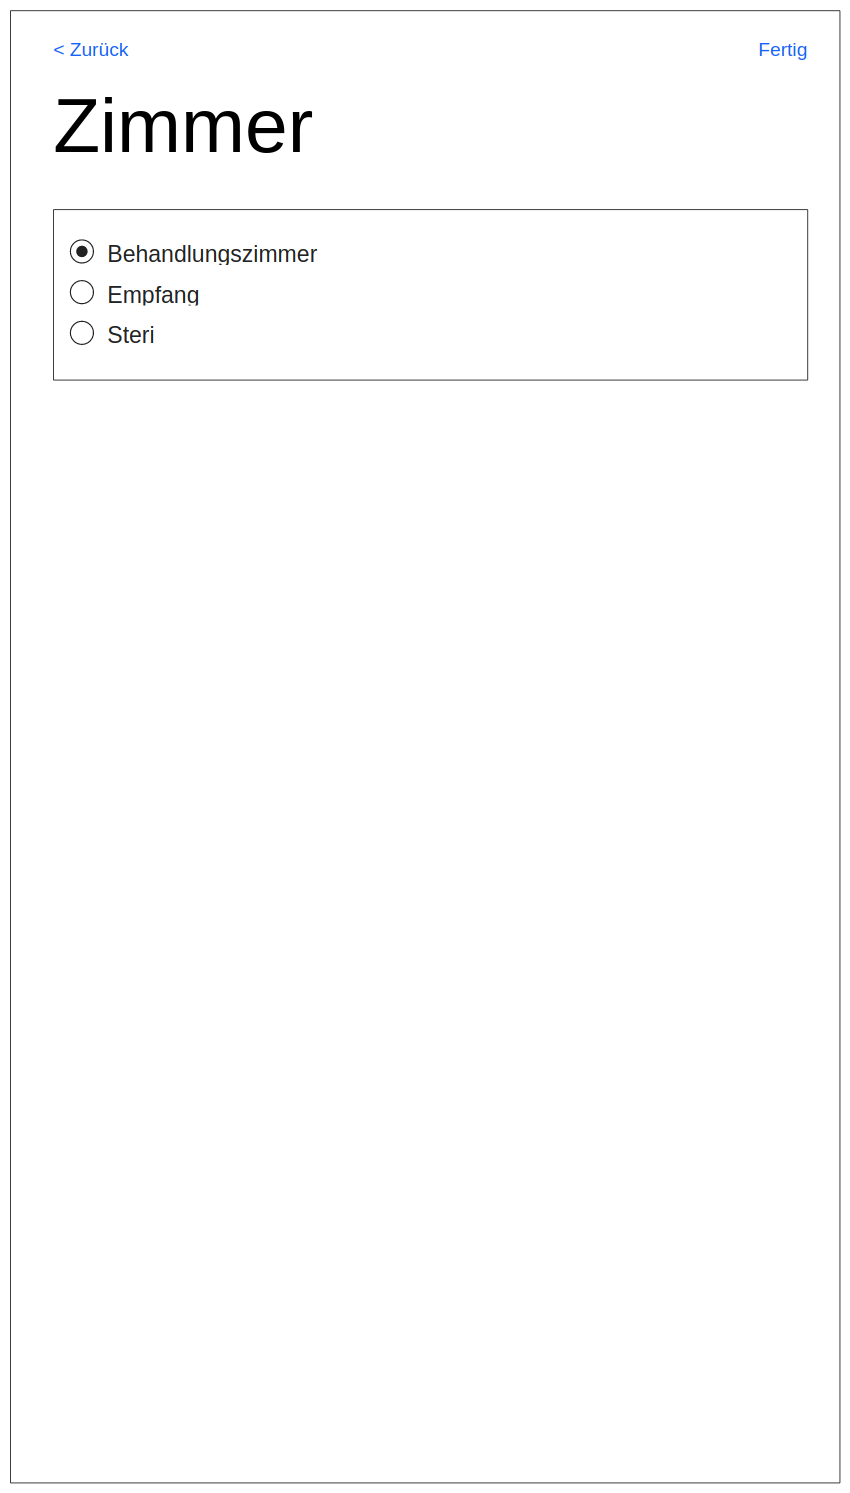
\includegraphics[width=\textwidth]{/home/joshua/FHNW/dev/IP6/IP6_Bachelorarbeit_Bericht_Cloudbasiertes_Praxisrufsystem/src/graphics/mockups/mockup_clientselect}}
        \caption{Mockup Zimmerwahl}
    \end{minipage}\label{fig:Mockups-Login-ClientSelection}
\end{figure}

Nach dem Eingeben der Anmeldedaten werden Praxismitarbeitende aufgefordert, die gewünschte Konfiguration auszuwählen.
Die Ansicht besteht aus einem Seitentitel und einer Liste zur Auswahl der gewünschten Konfiguration.
In der Auswahl sind alle Zimmer zu sehen, welche dem Benutzer zur Verfügung stehen.
Diese Konfigurationen müssen vor der Anmeldung im Admin UI erfasst und dem Benutzer zugewiesen werden.
In der Kopfzeile sind die Schaltflächen ''Zurück'' und ''Fertig'' zu sehen.
Die Schaltfläche ''Zurück'', bricht die Anmeldung ab und führt zurück zur Eingabe der Logindaten.
Die Schaltfläche ''Fertig'' bestätigt die Auswahl und leitet zur Hauptansicht weiter.
Wird bestätigt, ohne dass ein Zimmer angewählt ist, wird dem Benutzer eine Fehlermeldung angezeigt und nicht zur Hauptansicht weitergeleitet.

Die Hauptansicht der Applikation gliedert sich in die Bereiche Home, Inbox und Einstellungen.
Zwischen den drei Bereichen kann über eine Leiste am unteren Ende des Bildschirms navigiert werden.
Die Ansicht Home zeigt dem Benutzer die Buttons, über welche er Benachrichtigungen versenden und Anrufe in der Gegensprechanlage starten kann.
Wird ein Anruf gestartet, wird die Ansicht für aktive Anrufe angezeigt.
Diese zeigt dem Benutzer den Titel des gestarteten Anrufs, sowie eine Liste aller Teilnehmer zusammen mit dem Verbindungsstatus jedes Teilnehmers.
Der Titel des Anrufes entspricht dem Anzeigetext des verwendeten Buttons für ausgehende Anrufe und dem Namen des Anrufers für empfangene Anrufe.
Neben den Anrufinformationen zeigt die Ansicht für aktive Anrufe drei Buttons.
Über diese können Mikrofon und Lautsprecher des eigenen Gerätes stumm geschaltet werden.
Weiter kann der Anruf über einen roten Button am rechten Rand beendet werden.
Nach einem beendeten Anruf wird automatisch zu der zuvor angezeigten Ansicht navigiert.

\begin{figure}[h]
    \centering
    \begin{minipage}[b]{0.4\textwidth}
        \fbox{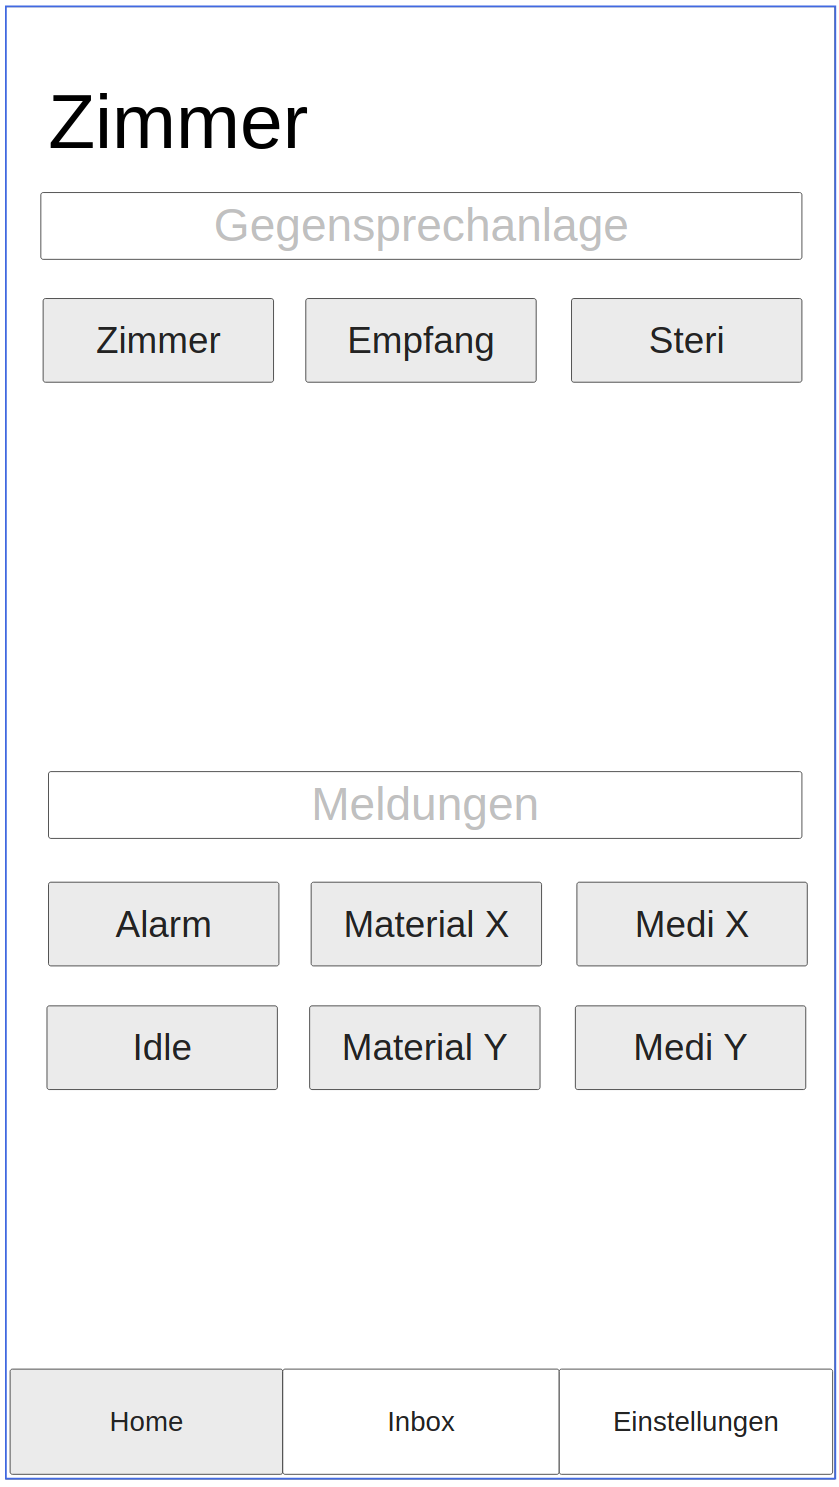
\includegraphics[width=\textwidth]{/home/joshua/FHNW/dev/IP6/IP6_Bachelorarbeit_Bericht_Cloudbasiertes_Praxisrufsystem/src/graphics/mockups/mockup_intercom}}
        \caption{Mockup Home}
    \end{minipage}
    \hfill
    \begin{minipage}[b]{0.4\textwidth}
        \fbox{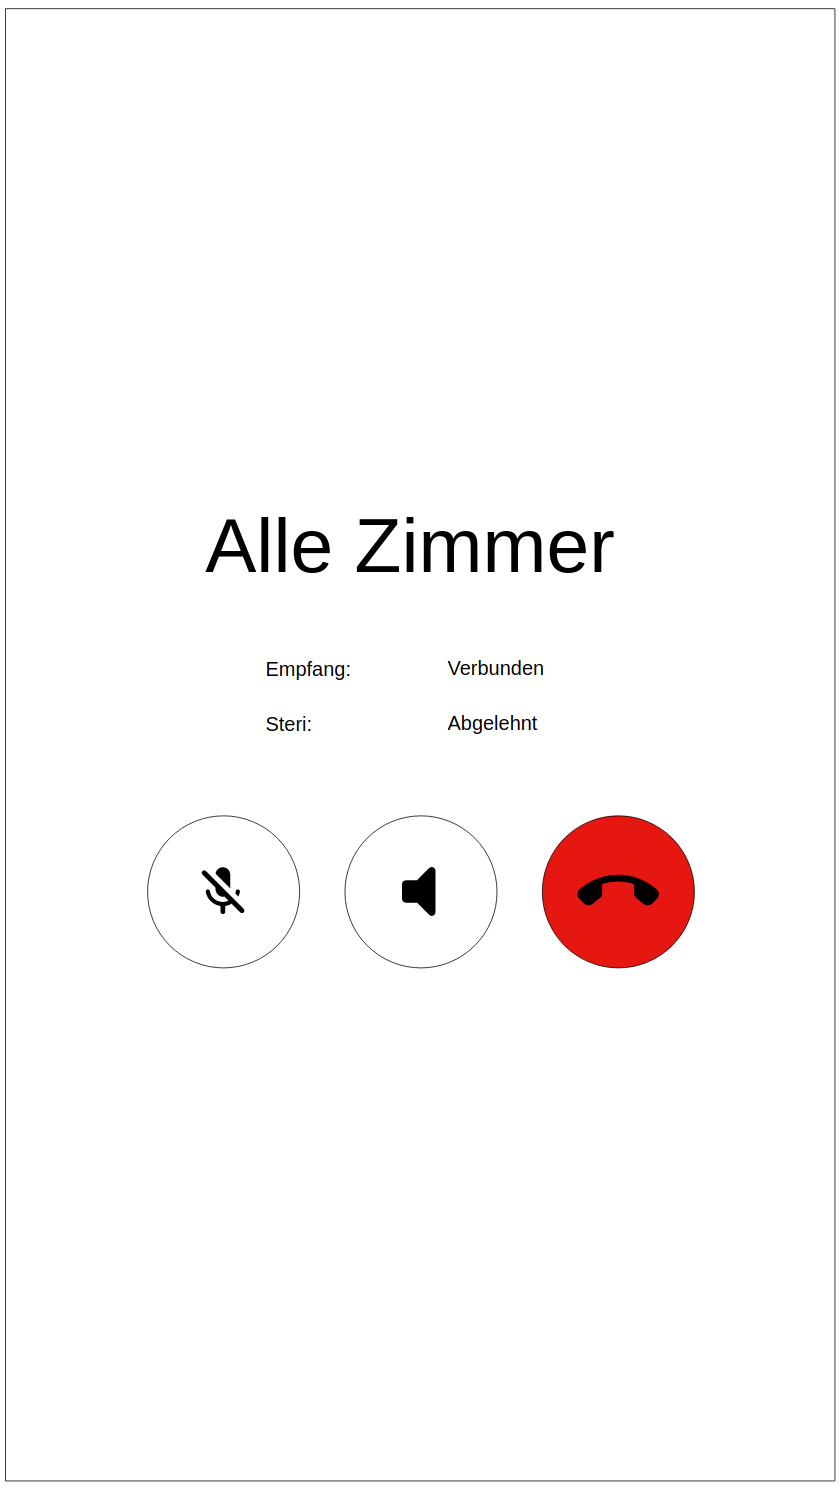
\includegraphics[width=\textwidth]{/home/joshua/FHNW/dev/IP6/IP6_Bachelorarbeit_Bericht_Cloudbasiertes_Praxisrufsystem/src/graphics/mockups/mockup_call}}
        \caption{Mockup Aktiver Anruf}
    \end{minipage}\label{fig:Mockups-Home-ActiveCall}
\end{figure}

Der Bereich Inbox zeigt eine Liste der empfangenen Benachrichtigungen sowie der empfangenen und verpassten Anrufe.
Für alle Elemente in der Inbox wird der Name des Senders als Überschrift angezeigt.
Darunter werden weitere Detailinformationen beschrieben.
Für Benachrichtigungen beinhaltet dies den Textinhalt der Benachrichtigungen.
Bei Anrufen beschrieben ob, es sich um einen empfangenen, verpassten oder abgelehnten Anruf handelt.
Einträge für Benachrichtigungen sowie verpasste und abgelehnte Anrufe müssen durch eine Wischgeste quittiert werden.
Die Funktionsweise der Quittierung wird aus dem bestehenden Mobile Client übernommen.
Quittierte Meldungen werden aus der Inbox entfernt und nicht mehr angezeigt.
Ein Quittieren von Meldungen und Anrufen passiert ausschliesslich lokal in der iOS Applikation.
Der Empfänger wird nicht über die Quittierung informiert~\cite{ip5}.

Es muss sichergestellt werden, dass verpasste Benachrichtigungen und Anrufe nicht übersehen werden.
Dazu wird im Abstand von 60 Sekunden geprüft, ob unquittierte Benachrichtigungen oder Anrufe in der Inbox vorhanden sind.
Ist dies der Fall, wird ein Erinnerungston abgespielt und eine Benachrichtigung angezeigt.
Dieser Mechanismus wird in Kapitel 7.2.4 weiter beschrieben.

\begin{figure}[h]
    \centering
    \begin{minipage}[b]{0.4\textwidth}
        \fbox{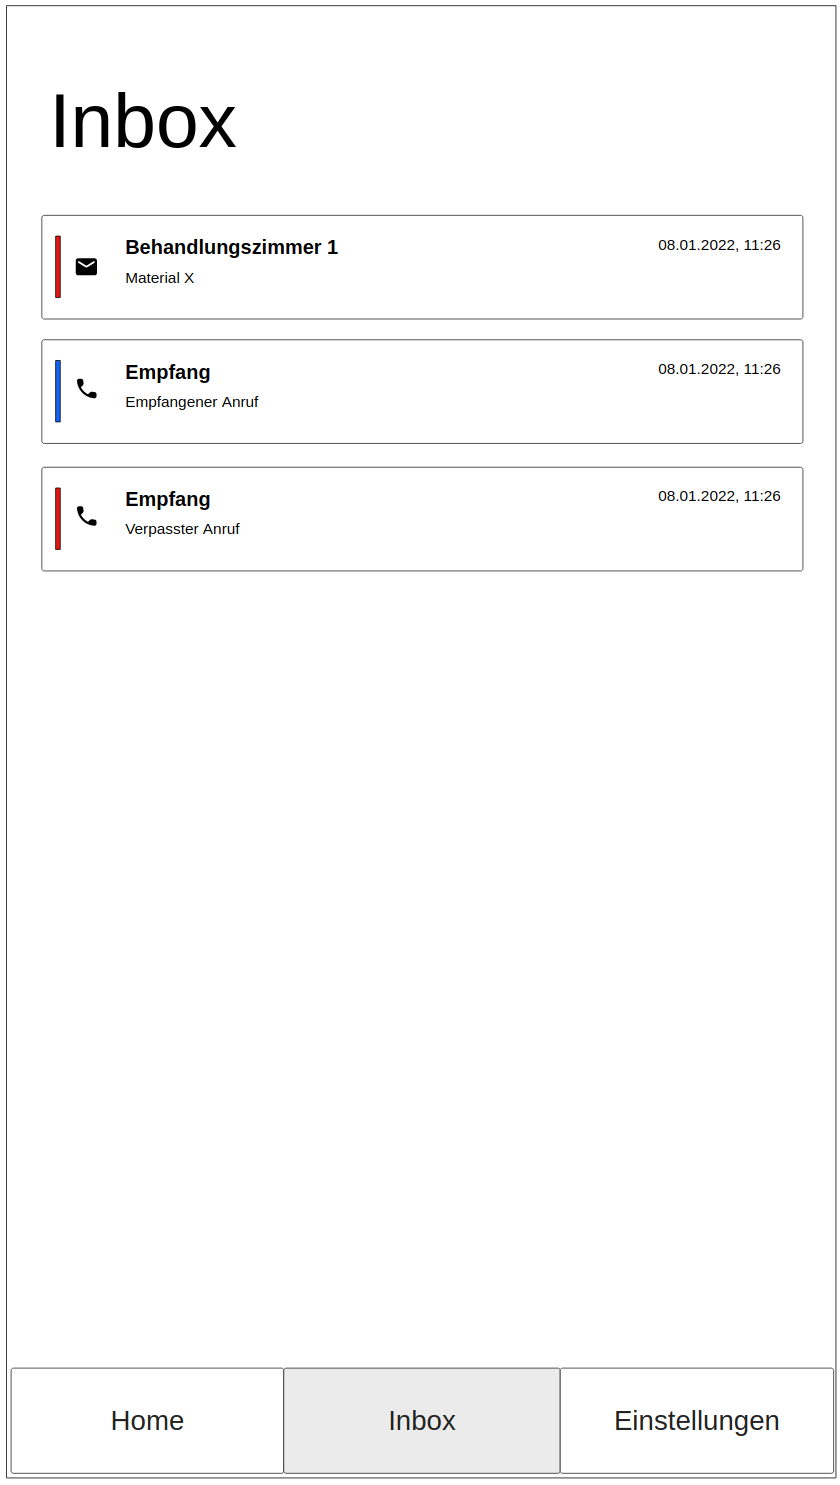
\includegraphics[width=\textwidth]{/home/joshua/FHNW/dev/IP6/IP6_Bachelorarbeit_Bericht_Cloudbasiertes_Praxisrufsystem/src/graphics/mockups/mockup_inbox}}
        \caption{Mockup Inbox}
    \end{minipage}
    \hfill
    \begin{minipage}[b]{0.4\textwidth}
        \fbox{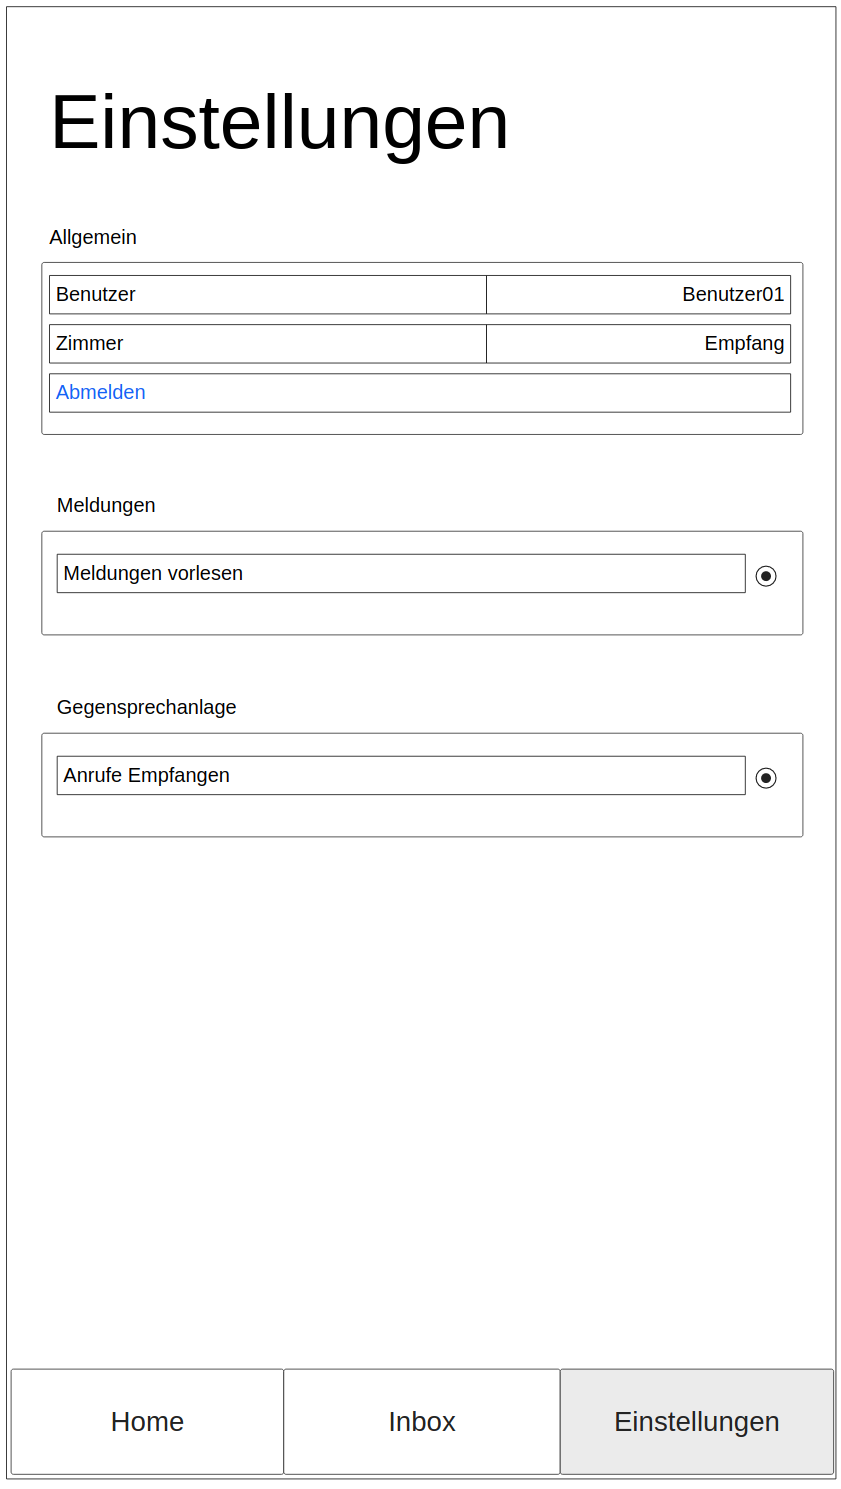
\includegraphics[width=\textwidth]{/home/joshua/FHNW/dev/IP6/IP6_Bachelorarbeit_Bericht_Cloudbasiertes_Praxisrufsystem/src/graphics/mockups/mockup_settings}}
        \caption{Mockup Einstellungen}
    \end{minipage}\label{fig:Mockups-Inbox-Settings}
\end{figure}

Abbildung 7.8 zeigt den Bereich Einstellungen.
Der Bereich Einstellungen zeigt den aktuellen Benutzernamen und die gewählte Konfiguration.
Über die Schaltfläche Abmelden, können sich Praxismitarbeitende aus der Applikation abmelden.
Die Schaltfläche Benachrichtigungen vorlesen ist standardmässig aktiviert.
Wird die Option deaktiviert, werden Benachrichtigungen nie vorgelesen.
Die Schaltfläche Anrufe empfangen ist ebenfalls standardmässig aktiviert.
Wird diese Option deaktiviert, werden alle empfangenen Anrufe automatisch abgelehnt und stattdessen eine Benachrichtigung angezeigt.
Ausgehende Anrufe können auch getätigt werden, wenn diese Option aktiviert ist.

\subsubsection{Anbindung Cloudservice API}

Der Mobile Client muss an die API des Cloudservices angebunden werden.
Es wird eine Anbindung an die Domäne Configuration zur Anmeldung und Auswahl des gewünschten Zimmers und an die Domäne Notification zum Versenden von Benachrichtigungen benötigt.
Die Schnittstellen dieser Domänen stehen als Http Endpunkte zur Verfügung.
In diesem Unterkapitel wird beschrieben, wie Http-Anfragen an die Cloudservice API in den nativen iOS Client integriert werden.
Das Abrufen von Sprachdaten und die Anbindung an die Signaling Instanz werden in den Kapiteln 7.3 und 7.4 beschrieben.

Die Basisbibliothek für iOS Entwicklung bietet die Klasse URLSession, über welche Netzwerkaufrufe getätigt werden können.
Über URLSession.shared steht eine Standard-Instanz zur Verfügung, über welche Netzwerkanfragen verarbeitet werden können~\cite{ios_urlsession}.
Die Klasse UrlRequest ermöglicht es, Http-Request für eine URL mit Header und Body zu erstellen~\cite{ios_urlrequest}.
Um die Integration dieser Klassen in die Applikation zu vereinfachen, wird ein zentraler Service mit dem Namen PraxisrufApi erstellt.
Dieser kapselt das Erstellen, Befüllen und Absetzten der nötigen UrlRequest Instanzen.
Er bietet öffentliche Methoden für die Http Verben Get, Post und Delete an.
Über diese können Http-Requests mit der jeweiligen Methode abgesetzt werden.
Zur Darstellung von Fehlern wird die Enum PraxisrufApiError erstellt.
Diese definiert Fehlerkategorien und wird von PraxisrufApi verwendet, um Aufrufern das Fehlschlagen einer Anfrage mitzuteilen.
Das Klassendiagramm in Abbildung 7.9 zeigt den Aufbau des Service PraxisrufApi\@.

\begin{figure}[h]
    \centering
    \begin{minipage}[b]{0.8\textwidth}
        \fbox{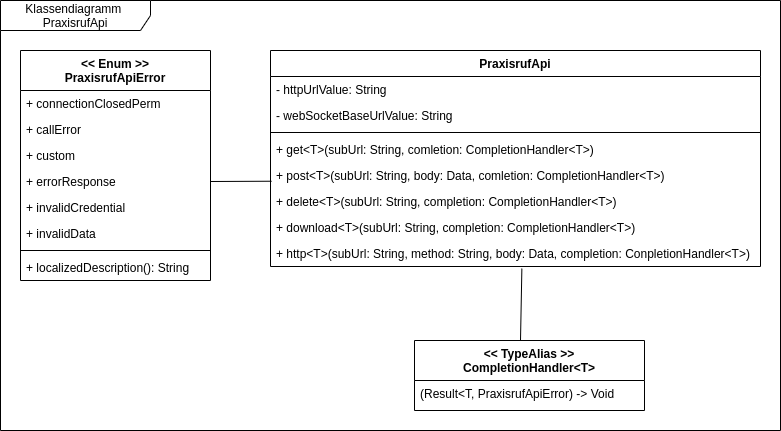
\includegraphics[width=\textwidth]{graphics/diagramms/Class_PraxisrufAPI}}
        \caption{Klassendiagramm PraxisrufApi}
    \end{minipage}
\end{figure}

Die Basis-URL für Http-Anfragen wird in der Konfiguration der iOS Applikation definiert.
Der PraxisrufApi Service lädt diese und verwendet sie für alle Abfragen, die abgesetzt werden.
Alle öffentlichen Methoden von PraxisrufApi nehmen einen Parameter ''subUrl'' als String entgegen.
Dieser String wird der Basis-URL angehängt.
Die Methoden Post nimmt zudem einen optionalen Parameter von Typ Data entgegen.
Dieser definiert den Inhalt des Request Bodies.
Mit diesen Informationen kann der Http Request erstellt und versendet werden.

Sämtliche öffentlichen Methoden des PraxisrufApi Service nehmen weiter einen Parameter mit dem Namen completion entgegen.
Dabei handelt es sich um eine Funktion, welche beim Erfolg oder Fehlschlagen der Http-Anfragen ausgeführt wird.
Als Parameter dieser Funktion wird immer der Typ Result$<$T, PraxisrufApiError$>$ verwendet.
Bei Result handelt es sich um einen Wrapper Typen welcher entweder das Resultat einer Abfrage oder ein Fehlerobjekt beinhaltet~\cite{ios_result}.
Im Fehlerfall wird das Result mit einem PraxisrufApiError Objekt erstellt.
Im Erfolgsfall wird es mit den Daten aus dem Body der Http-Antwort befüllt.
Zur Darstellung dieser Daten wird der generische Typ T verwendet.
Der Typ wird vom Aufrufer von PraxisrufApi definiert und kann grundsätzlich beliebig sein.
Er muss aber das Protokoll Decodable aus der iOS Standardbibliothek implementieren.
Decodable Instanzen können von einer JSON-String-Repräsentation in ein Swift-Objekt konvertiert werden~\cite{ios_decodable}.
So kann das Resultat im Erfolgsfall aus der Response generiert und an, dass Callback übergeben werden.
Dadurch kann die Konvertierung generisch in im PraxisurfApi-Service behandelt werden.

Anhand des Inhalts der Result-Instanz kann geprüft werden, ob die Anfrage erfolgreich war.
Das Resultat kann entsprechend verarbeitet werden.
Diese Prüfung und Verarbeitung findet innerhalb der completion-Funktion statt.
Dieser Ansatz ermöglicht es im PraxisrufApi-Service ausschliesslich Http-Anfragen zu senden und die entsprechenden Antworten entgegenzunehmen.
Der Api Service behandelt damit ausschliesslich die technische Anbindung an die API des Cloudservice.
Er muss keine fachliche Logik implementieren und kann generisch für alle Anwendungen wiederverwendet werden.

Requests die über den PraxisrufApi-Service erstellt werden, werden automatisch authentisiert.
Dazu lädt der Service die hinterlegten Credentials aus dem KeyStore von iOS.
Das Token wird verwendet, um einen entsprechenden Authorization-Header zu generieren.
Der generierte Authorization Header wird der Http-Anfrage angefügt.
Ist kein Token vorhanden, wird keine Anfrage abgesetzt.
Es wird direkt die completion-Funktion mit dem Fehler PraxisrufApiError.invalidCredential aufgerufen.

Mit dieser Lösung steht ein Service zur Verfügung, über welchen Http-Anfragen einfach in eine iOS App integriert werden können.
Dank der generischen Methoden im PraxisrufApi-Service können neue Calls einfach hinzugefügt werden, ohne das Boilerplate-Code wiederholt werden muss.
Durch die completion-Funktionen kann die fachliche Verarbeitung von Http-Anfragen vom Aufrufer definiert werden.

Um die Verwendung der Cloudservice API weiter zu vereinfachen, wird der PraxisrufApi Service um sprechende Methoden für die nötigen Abfragen erweitert.
Dazu wird pro Domäne eine Extension-Klasse erstellt.
Diese fügt Methoden mit sprechenden Namen für die angesprochene Funktionalität hinzu und kapseln die Verwendung der Get, Post und Delete Methoden.

Der PraxisrufApi-Service ermöglicht es Abfragen an die Cloudservice API abzusetzen.
Die Resultate dieser Abfragen müssen in der Benutzeroberfläche angezeigt werden können.
Es wird pro Domäne ein weiterer Service geschrieben, welche den Aufruf des API Services kapselt.
Dieser Service bietet Methoden, über welche der PraxisrufApi Service angesprochen werden kann.
View-Komponenten können diese Services nutzen, um durch Benutzereingaben ausgelöste Anfragen an die Cloudservice Api zu senden.
Resultate und Fehler aus Anfragen an den Cloudservice werden in diesen Services als Instanzvariablen gehalten.
Die View-Komponenten können lesend auf diese Variablen zugreifen, um die entsprechenden Resultate oder Fehler anzuzeigen.

\subsubsection{Anbindung Messaging Service}

Um Benachrichtigungen empfangen zu können, muss Firebase Cloud Messaging an die native iOS Applikation angebunden werden.
Firebase bietet eine Bibliothek mit welcher Firebase Cloud Messaging in iOS Clients integriert werden kann~\cite{firebase_ios}.
Diese Integration kann allerdings nicht mit dem Mitteln von SwiftUI implementiert werden.
Dies liegt daran, dass für das Empfangen von Benachrichtigungen und das Anzeigen von Push-Benachrichtigungen Integration mit dem Benachrichtigungszenter des Betriebssystem notwendig ist.
Diese Integration kann bis heute nur über AppDelegates umgesetzt werden.
SwiftUI Applikationen können oft ohne AppDelegates implementiert werden.
Sobald aber Integration mit dem Betriebssystem notwendig ist, müssen AppDelegates verwendet werden.
Dazu können AppDelegates bei der Initialisierung der Applikation registriert werden.

Zur Anbindung von Firebase Cloud Messaging wird dementsprechend ein AppDelegate implementiert.
Die Logik des Delegates wird dabei auf das minimal Nötige reduziert.
Der AppDelegate selbst ist für die direkte Kommunikation mit Firebase verantwortlich und muss empfangene Daten an Betriebssystem und SwiftUI Applikation übergeben.
Fachliche Logik wird nicht im AppDelegate, sondern in der SwiftUI Applikation ausgeführt.
Dies ermöglicht es die Anbindung des Messaging Service im AppDelegate zu kapseln.
Sollte Firebase Cloud Messaging in Zukunft durch einen anderen Anbieter ersetzt werden, muss damit ausschliesslich die Logik im AppDelegate angepasst werden.
Diese Trennung stellt sicher, dass die Fachlogik vollständig mit SwiftUI implementiert werden kann.
Der AppDelegate beinhaltet lediglich die Teile, welche aus technischen Gründen nicht mit SwiftUI umgesetzt werden können.

Um Benachrichtigungen von Firebase Cloud Messaging empfangen zu können, muss der AppDelegate folgende Funktionalität umsetzen.
Beim Start der Applikation muss sich der Mobile Client beim Messaging Service registrieren.
Nach der Registrierung wird für den Mobile Client ein Token generiert, welches den Client eindeutig beim Messaging Service identifiziert.
Der AppDelegate muss, darauf reagieren und das erneuerte Token an die Applikation übergeben.

Für die Verarbeitung von Benachrichtigungen muss der AppDelegate Benachrichtigungen im Vordergrund empfangen und dem Betriebssystem zur Anzeige übergeben.
Die Informationen aus der empfangenen Benachrichtigung müssen anschliessend an die Applikation übergeben werden.
Benachrichtigungen, die im Hintergrund empfangen werden, müssen an das Betriebssystem übergeben und angezeigt werden.
Sobald die Applikation wieder in den Vordergrund tritt, müssen die Daten an die Applikation zur weiteren Verarbeitung übergeben werden.

\subsubsection{Benachrichtigungen prüfen}

Der bestehende Mobile Client prüft in regelmässigen Abständen, ob ungelesene Benachrichtigungen in der Inbox vorhanden sind.
Wenn ungelesene Benachrichtigungen gefunden werden, wird ein Benachrichtigungston abgespielt.
Im Mobile Client der Vorgängerlösung findet diese Prüfung nur statt, wenn die Applikation in Vordergrund aktiv ist.
Diese Funktion wird in der nativen iOS Applikation übernommen.

Für die Umsetzung der Erinnerungsfunktion werden zwei Services definiert.
Erstens wird eine Inbox erstellt, welche eine Liste der aktuellen Benachrichtigungen führt.
Zweitens wird ein InboxReminderService implementiert.
Dieser prüft den Inhalt der Inbox und sucht nach unquittierten Elementen, welche älter als eine Minute sind.
Werden solche Elemente gefunden, wird eine Benachrichtigung angezeigt und ein Benachrichtigungston abgespielt.
Die regelmässige Prüfung der Inbox wird mit der Timer-Klasse der iOS Standardbibliothek umgesetzt.
Über diese ist es möglich auf einer View in regelmässigen Abständen Events auszulösen~\cite{ios_timer}.
Ein solcher Timer wird auf der Hauptansicht für angemeldete Benutzer registriert.
Der Timer löst alle 60 Sekunden die Prüfung des InboxReminderService aus.

Die Prüfung von Benachrichtigungen im Hintergrund wird im Rahmen dieses Projektes nicht umgesetzt.
Für künftige Erweiterungen ist es möglich diese Funktion zu implementieren.
Um dies zu ermöglichen, müssen Benachrichtigungen auf dem Gerät persistiert werden.
So stehen die Daten auch zur Verfügung, wenn die Applikation nicht gestartet ist.
Weiter muss ein Hintergrundtask implementiert und registriert werden~\cite{ios_bgtaskscheduler}, welcher die persistierten Daten lädt und die darauf die Prüfung des InboxReminderService ausführt.

\subsubsection{Security}

In einem Praxisrufsystem muss die sichere Übertragung von Daten gewährleistet sein.
Die dazu definierten Konzepte werden aus dem Vorgängerprojekt übernommen.

Alle Daten zwischen den Services müssen über verschlüsselte Verbindungen ausgetauscht werden.
HTTP Anfragen CloudService API erfolgen ausschliesslich über HTTPS\@.
Alle Anfragen an die API des Cloudservice müssen zudem mit einem Json Web Token (JWT) authentifiziert sein.
Praxismitarbeitende werden durch den Cloudservice mittels Basic Authentication authentifiziert.
Bei der Anmeldung mit Benutzername und Passwort liefert der Cloudservice ein JWT, welches vom Client für weitere Anfragen verwendet wird.
Sowohl die Credentials für die Basic Authentication als auch das JWT Token werden durch die iOS Applikation im Keystore des Betriebssystems gespeichert~\cite{ip5}.
Das Token wird regelmässig erneuert, indem die Basic Authentication mit den gespeicherten Credentials wiederholt wird.
Der Ablauf für Authentifizierung wird damit unverändert aus dem Vorgängerprojekt übernommen.

\clearpage

\subsubsection{Servicemodell}

Dieses Kapitel gibt einen Überblick zu den Services welche in der nativen iOS Applikation beinhaltet werden.
Abbildung 7.10 zeigt das vollständige Modell der implementierten Services.
Diese Darstellung beinhaltet die Services, welche in den Kapiteln 7.2 bis 7.4 beschrieben werden.
View- und Model-Komponenten werden hier nicht dargestellt.

\begin{figure}[h]
    \centering
    \begin{minipage}[b]{1\textwidth}
        \fbox{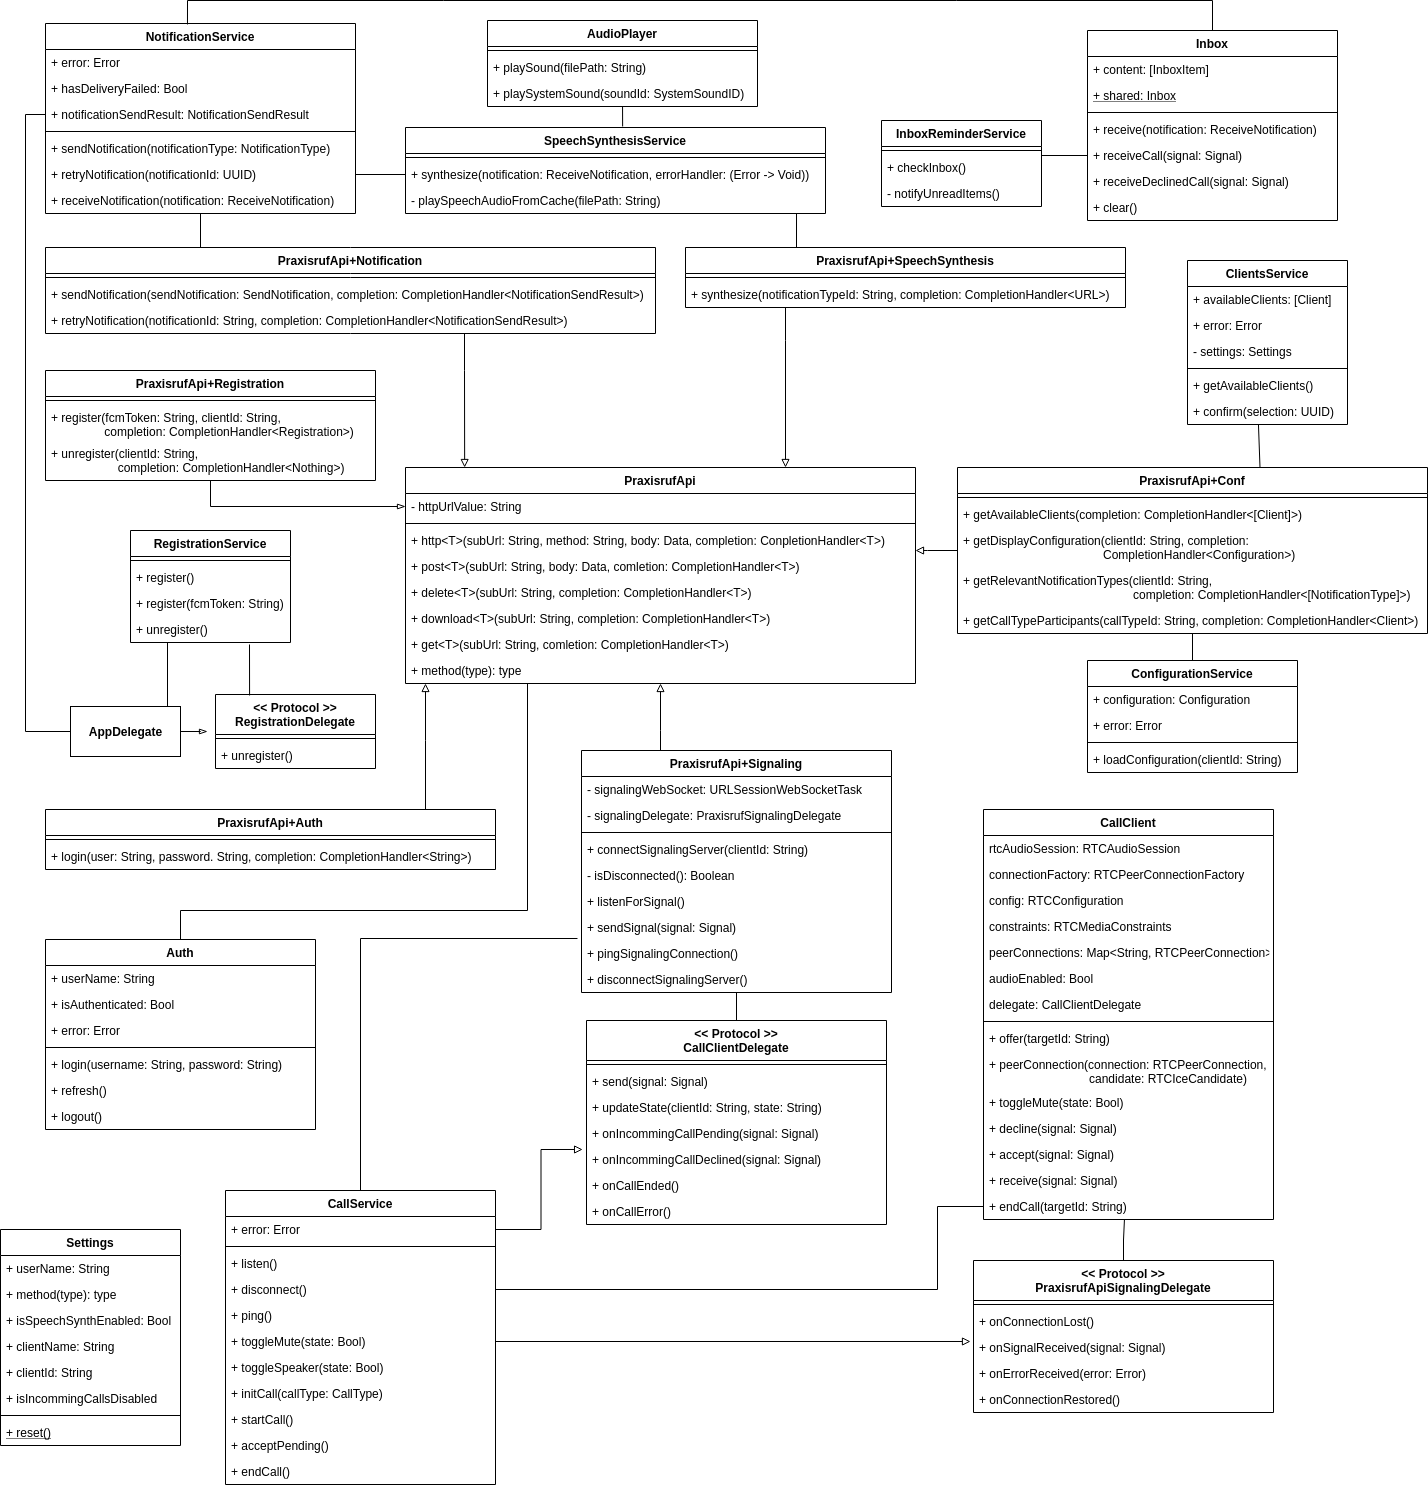
\includegraphics[width=\textwidth]{/home/joshua/FHNW/dev/IP6/IP6_Bachelorarbeit_Bericht_Cloudbasiertes_Praxisrufsystem/src/graphics/diagramms/Class_Mobile_Client_Services}}
        \caption{Klassendiagramm - App Services}
    \end{minipage}
\end{figure}

Die Klasse Settings wird verwendet um die Konfiguration des Benutzers zu verwalten.
Sie bietet Getter und Setter für alle Properties.
Nach dem setzten eines Wertes, wird dieser über die Komponente UserData aus der iOS Standardbibliothek persistiert.
Die Verwendungen der Settings-Klasse sind in Abbildung 7.10 nicht dargestellt, um die Übersichtlichkeit zu wahren.

\clearpage

\subsection{Sprachsynthese}

Dieses Kapitel beschreibt die Integration von Sprachsynthese in Praxisruf.
Der Fokus liegt dabei auf den Abläufen zum Empfangen von Benachrichtigungen und dem Abrufen der Sprachdaten.
Der Empfang von Benachrichtigungen wird so erweitert, dass der Inhalt empfangener Benachrichtigungen automatisch vorgelesen wird.

\subsubsection{Konfiguration}

Benachrichtigungen für Praxisruf können über das Admin UI konfiguriert werden.
Es können pro Benachrichtigung Titel, Inhalt, Beschreibung sowie ein Anzeigetext erfasst werden.
Der Anzeigetext wird als Text des Buttons verwendet, über welchen die Benachrichtigung versendet wird.
Diese Konfiguration wird über die Entität NotificationType verwaltet.
Neu soll auch konfiguriert werden können, ob eine Benachrichtigung für die Sprachsynthese relevant ist.
Dazu wird die Entität NotificationType um ein boolean Flag mit dem Namen ''isTextToSpeech'' erweitert.
Dieses Flag wird beim Versenden einer Benachrichtigung mitgesendet und kann vom Empfänger überprüft werden.
Wenn das Vorlesen von Benachrichtigungen in den lokalen Einstellungen und das Flag auf der Benachrichtigung aktiviert sind, wird die Benachrichtigungen vorgelesen.
Abbildung 7.11 zeigt einen Ausschnitt aus dem Entity Relationship Diagramm der Domäne Configuration.
Dabei sind die Felder, welche für die Sprachsynthese ergänzt werden, grün markiert.

\begin{figure}[h]
    \centering
    \begin{minipage}[b]{0.6\textwidth}
        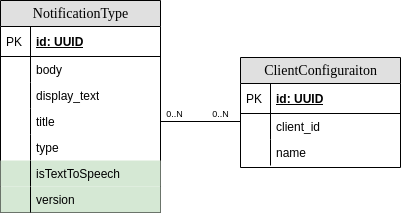
\includegraphics[width=\textwidth]{/home/joshua/FHNW/dev/IP6/IP6_Bachelorarbeit_Bericht_Cloudbasiertes_Praxisrufsystem/src/graphics/diagramms/erd_t2s_v01.drawio}
        \caption{ERD Ausschnitt - Konfiguration Sprachsynthese}
    \end{minipage}
\end{figure}

Neben dem Feld ''isTextToSpeech'', wird die NotificationType-Entität um ein weiteres Feld ''version'' erweitert.
Das Versionsfeld beinhaltet eine Ganzzahl, welche mit jeder Änderung inkrementiert wird.
Der Inhalt dieses Felds wird ebenfalls beim Versenden von Benachrichtigungen mitgesendet.
Auf Client-Seite wird diese Information zur Implementierung eines Cache verwendet.

\subsubsection{Anbindung von Sprachsynthese in Cloudservice}

Dieses Kapitel beschreibt, wie Amazon Polly an den Cloudservice angebunden wird, um das Vorlesen von Benachrichtigungen zu ermöglichen.

Die Anbindung an Amazon Polly erfolgt zentral im Cloudservice.
Sämtliche Anfragen an Amazon Polly werden durch den Cloudservice gemacht.
Empfänger von Benachrichtigungen senden keine direkten Anfragen an Amazon Polly.
Sie kommunizieren stattdessen mit dem Cloudservice.
Dieser führt die Anfrage an Amazon Polly aus und gibt die Resultate an den Anfrager zurück.

Für die Anbindung von Amazon Polly wird der Cloudservice um ein Modul mit dem Namen ''Speech Synthesis'' erweitert.
Dieses Modul muss unabhängig von allen anderen Domänen-Modulen des Cloudservice umgesetzt werden.
Werden Daten aus einer anderen Domäne benötigt, muss die Kommunikation über die API des entsprechenden Moduls gehen.
Diese Trennung ermöglicht es, das Modul in Zukunft einfach aus dem Cloudservice auszubauen und als eigenständigen Microservice zu betreiben.

Die Abhängigkeit zu Amazon Polly als Anbieter soll weitmöglichst minimiert werden.
So kann bei Bedarf einfacher auf einen anderen Provider gewechselt werden.
Um dies zu ermöglichen wird das Interface SpeechSynthesisService definiert.
Dieses gibt eine Methode vor, welche eine InputStreamResource zurückgibt.
Sie nimmt zwei Universal Unique Ids (UUID) als Parameter entgegennimmt.
Der erste Parameter entspricht der technischen Identifikation des zu synthetisierenden Benachrichtigungstypes (NotificationType).
Der zweite Parameter entspricht der Identifikation des Senders der Benachrichtigung.
Die InputStreamResource muss die synthetisierten Sprachdaten enthalten.
Dieses Interface wird von der Komponente, welche die Schnittstelle nach aussen bietet verwendet.
Um einen Anbieter für Sprachsynthese anzubinden, kann dieses Interface implementiert werden und der Schnittstelle zur Verfügung gestellt werden.
Das Klassendiagramm in Abbildung 7.12 gibt einen Überblick über den Aufbau des Moduls Speech Synthesis.

\begin{figure}[h]
    \centering
    \begin{minipage}[b]{1\textwidth}
        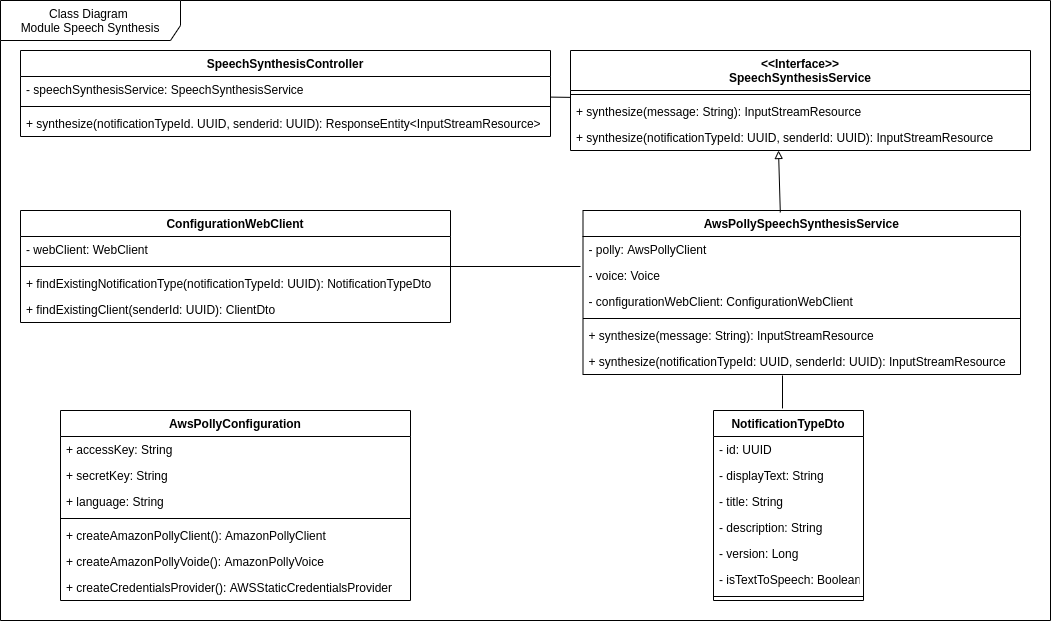
\includegraphics[width=\textwidth]{/home/joshua/FHNW/dev/IP6/IP6_Bachelorarbeit_Bericht_Cloudbasiertes_Praxisrufsystem/src/graphics/diagramms/Class_AWS_Polly_Configuration_V02}
        \caption{Klassendiagramm - Modul SpeechSynthesis}
    \end{minipage}
\end{figure}

Für die Anbindung des Providers Amazon Polly wird das Interface SpeechSynthesisService mit der Klasse AwsPollySpeechSynthesisService implementiert.
Amazon stellt einen Java Bibliothek für Amazon Polly zur Verfügung, welcher diese Anbindung ermöglicht~\cite{aws_polly_sdks}.
Diese Bibliothek bietet alle Klassen, die für die Anbindung an Amazon Polly nötig sind.
Sie wird bei in AwsPollySpeechSynthesisService verwendet, um Amazon Polly anzubinden.

Die Anbindung von Amazon Polly benötigt drei Komponenten.
Als Erstes muss eine Instanz von AWSStaticCredentialsProvider zur Verfügung gestellt werden.
Diese liefert die Credentials, welche das System berechtigen, Anfragen an Amazon Polly zu senden.
Als Zweites muss eine Voice konfiguriert werden.
Die Voice definiert Sprache und Stimme, welche für die Sprachausgabe verwendet wird.
Letztlich muss eine Instanz von AmazonPollyClient konfiguriert werden.
Dieser Client wird verwendet, um Anfragen an Amazon Polly zu senden.
Er verwendet den zuvor konfigurierten CredentialsProvider, um die Anfrage mit den entsprechenden Credentials zu ergänzen.
Die zuvor konfigurierte Voice wird bei Anfragen an Amazon Polly mitgesendet, damit die Daten mit den gewünschten Parametern synthetisiert werden.

Der Cloudservice ist als Java-Applikation mit Spring Boot umgesetzt.
Dies ermöglicht es, die notwendigen Komponenten in einer Spring Konfigurationsklasse zu konfigurieren und als Spring Beans zu instanziieren.
Über die Dependency Injection von Spring werden diese Komponenten dem AwsPollySpeechSynthesisService übergeben werden.

Werte, welche für die technische Konfiguration notwendig sind, werden aus der Konfigurationsdatei application.yml geladen.
Sprache und Region werden sich im Rahmen dieses Projektes nie ändern und beinhalten keine sensitiven Informationen.
Sie werden deshalb direkt in der Konfigurationsdatei definiert und mit dem Quellcode des Projektes verwaltet.
Als Credentials für die Anbindung dienen die zwei Schlüssel AccessKey und SecretKey.
Credentials werden nicht direkt in der Konfigurationsdatei gespeichert.
Stattdessen wird ein Platzhalter definiert, welcher die Werte für Credentials aus entsprechend benannten Umgebungsvariablen lädt.
Die Zugangsdaten müssen damit nicht mit dem Quellcode verwaltet werden.

\subsubsection{Sprachsynthese über Cloudservice API}

Endgeräte in Praxisruf müssen Sprachdaten über den Cloudservice beziehen können.
Das Modul Speech Synthesis stellt deshalb eine Schnittstelle zur Verfügung, über welche Sprachdaten abgefragt werden können.
Dabei ist es nicht möglich beliebige Textdaten in Sprachdaten zu verwandeln.
Stattdessen erlaubt die Schnittstelle die Abfrage von Sprachdaten für Inhalt und Sender einer Benachrichtigung.

Als Inhalt einer Benachrichtigung wird das Feld ''title'' aus der Entität NotificationType verwendet.
Der Name des Senders wird dem Feld ''name'' der Entität Client entnommen.
Beide Entitäten sind Teil des Moduls Configuration.
Die entsprechenden Daten müssen deshalb über die API des Configuration-Moduls geladen werden.
Um dies zu ermöglichen, werden die Identifikatoren der relevanten Entitäten zusammen mit Benachrichtigung versendet.

Der Endpunkt zum Bezug von Sprachdaten nimmt die zwei Parameter ''notificationTypeId'' und ''sender'' entgegen.
Diese müssen die technischen Identifikatoren der jeweiligen Entitäten beinhalten.
Anhand dieser Parameter werden der die benötigten Daten von der API des Configuration-Moduls geladen.
Anschliessend wird eine Anfrage an Amazon Polly gesendet um die Textdaten als Sprache zu synthetisieren.
Der zu synthetisierende Text setzt sich dabei aus Inhalt der Benachrichtigung und Name des Senders zusammen.
Die beiden Werte werden dabei durch ein Komma getrennt.
Dadurch wird eine Pause zwischen dem Vorlesen der einzelnen Werte eingefügt.
Die von Polly gelieferten Sprachdaten können anschliessend als Resultat zurückgegeben werden.

Der Endpunkt für die Abfrage von Sprachdaten im Cloud Service wird als Spring RestController umgesetzt.
Die Sprachdaten werden darin als Binärdaten mit Media Type ''audio/mp3'' im Body der Response zurückgegeben.
Der Endpunkt kann über Http-Get-Anfragen angesprochen werden.

\subsubsection{Security}

Anfragen an die API des Moduls Speech Synthesis müssen, wie alle Anfragen an die Cloudservice API, authentisiert werden.
Für die Authentisierung wird derselbe Mechanismus wie für Http-Anfragen in allen Cloudservice Modulen verwendet.
Über die Konfiguration des App-Moduls des Cloudservices wird die Authentifizierung aller Http-Requests überprüft.
Mit dieser Prüfung wird sichergestellt, dass ein gültiges JWT Token im Authentication Header der Anfrage vorhanden ist~\cite{ip5}.
Diese Prüfung wurde im Rahmen des Vorgängerprojektes umgesetzt und wird weiterverwendet.
Die entsprechenden Abläufe sind in dem Kapiteln 5.3.6 und 5.3.7 im Projektbericht ''IP5 Cloudbasiertes Praxisrufsystem'' dokumentiert~\cite{ip5}.

Um die Verschlüsselung der Übertragung von Sprachdaten und Anfragen zwischen Cloudservice und Mobile Client wird für die Übertragung ausschliesslich das Protokoll HTTPS verwendet.
Die Übertragung von Daten zwischen Cloudservice und Amazon Polly ist über Secure Sockets Layer (SSL) geschützt~\cite{aws_polly_encryption_in_transit}.

\subsubsection{Sprachsynthese in iOS App}

In der iOS App müssen empfangene Benachrichtigungen vorgelesen werden können.
Um dies zu ermögli-chen wird eine Anbindung an die Sprachsynthese-API des Cloudservice umgesetzt.
Dazu wird die in Kapitel 7.2 beschriebene Klasse PraxisrufApi erweitert.
Neben dem Abfragen von JSON Daten über HTTP Schnittstellen, muss diese für die Sprachsynthese auch das Herunterladen von Dateien unterstützten.
Dazu wird die Komponente URLSession aus der iOS Standardbibliothek verwendet.
Diese bietet mit URLSession.downloadTask die Möglichkeit Inhalte von einer URL herunterzuladen~\cite{ios_downloadtask}.

Der Service PraxisrufApi wird um eine Methode mit dem Namen ''download'' ergänzt.
Diese ist dafür verantwortlich, eine Anfrage für den Download mit Credentials aus dem iOS Keystore zu ergänzen und die Anfrage zu versenden.
Die Resultate der Anfrage und aufgetretene Fehler werden analog zu anderen Abfragen an eine Callback-Funktion übergeben.
Heruntergeladene Dateien werden von PraxisrufApi in einem temporären Verzeichnis gespeichert.
Das Resultat im Erfolgsfall ist deshalb nicht die heruntergeladene Datei selbst, sondern eine URL welche auf die Datei im temporären Verzeichnis zeigt.

Die Sprachsynthese für Benachrichtigungen muss automatisch ausgeführt werden, nachdem eine relevante Benachrichtigung empfangen wurde.
Der Empfang der Benachrichtigung findet über die Anbindung von Firebase Cloud Messaging im AppDelegate statt.
Die Benachrichtigung wird im AppDelegate empfangen und an die Applikation übergeben.
Die empfangene Benachrichtigung beinhaltet mit dem ''isTextToSpeech'' Flag, die Information, ob sie für die Sprachsynthese relevant ist.

Ist eine Benachrichtigung für Sprachsynthese relevant, werden die Sprachdaten dazu vom Cloudservice bezogen.
Dazu wird ein SpeechSynthesisService implementiert, welcher PraxisrufApi verwendet, um eine Anfrage an den Cloudservice zu senden.
Wurden die Daten erfolgreich geladen, kopiert der SpeechSynthesisService die heruntergeladenen Daten aus dem temporären Downloadverzeichnis in ein permanentes Verzeichnis.
Die Datei wird dabei unter dem Namen $NotificationTypeId.Version.SenderId$ gespeichert.
Sowohl NotificationTypeId als auch Version und SenderId können der empfangenen Benachrichtigung entnommen werden.
Nachdem die Sprachdatei unter dem neuen Namen gespeichert ist, wird ihr Inhalt abgespielt.

Die Namenskonvention für die gespeicherten Sprachdateien, erlaubt es ein Cache auf der Seite der iOS Applikation umzusetzen.
Bevor der SpeechSynthesisService eine Anfrage an den Cloudservice absetzt, prüft er, ob bereits eine Datei mit dem entsprechenden Namen vorhanden ist.
Ist dies der Fall, wird keine Anfrage an den Cloudservice gesendet und es wird die bereits gespeicherte Sprachdatei abgespielt.
Dieses Cache ermöglicht es Anfragen für Sprachsynthese zu minimieren und nach Änderungen trotzdem immer die aktuellsten Daten zu erhalten.

\clearpage

\subsubsection{Laufzeitsicht}

Dieses Kapitel beschreibt die Prozesse für das Vorlesen von Benachrichtigungen.
Dabei wird der Ablauf vom Versenden der Benachrichtigung bis hin zur Ausgabe der Sprachdaten auf Empfängerseite beschrieben.
Abbildung 7.13 stellt den Ablauf dem Empfangen einer Benachrichtigung aus Systemsicht dar.

Um eine Benachrichtigung zu versenden, sendet ein Mobile Client eine Anfrage an den Cloudservice.
Dieser lädt die gespeicherte Konfiguration und findet alle für die gewünschte Benachrichtigung relevanten Empfänger.
Anschliessend erstellt er für jeden Empfänger eine Benachrichtigung und versendet diese über den Messaging Service.
Der Messaging Service stellt die Benachrichtigungen an die Empfänger zu~\cite{ip5}.

Benachrichtigungen werden im Mobile Client über die Anbindung an den Messaging Service im AppDelegate empfangen.
Im AppDelegate werden die Informationen aus der empfangenen Benachrichtigung gelesen und in das interne Model der Mobile Client Applikation überführt.
Anschliessend wird die Benachrichtigung an das Betriebssystem übergeben damit auf dem Gerät ein Benachrichtigungston abgespielt und eine Push-Benachrichtigung angezeigt wird.
Daraufhin wird die Benachrichtigung im internen Model einem NotificationService übergeben.
Dieser fügt die empfangene Benachrichtigung in eine Inbox ein.
Ab diesem Moment ist die Benachrichtigung in der Inbox des Mobile Clients ersichtlich.

\begin{figure}[h]
    \centering
    \begin{minipage}[b]{0.8\textwidth}
        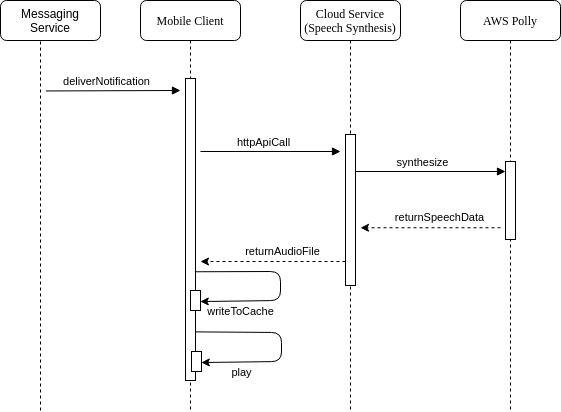
\includegraphics[width=\textwidth]{graphics/diagramms/Sequence_Speech_Synth_System}
        \caption{Sequenzdiagramm - Sprachsynthese auf Systemebene}
    \end{minipage}
\end{figure}


Nachdem eine empfangene Benachrichtigung der Inbox hinzugefügt wurde, wird geprüft ob Sprachsynthese in den lokalen Einstellungen aktiviert ist.
Ist diese deaktiviert, endet die Verarbeitung.
Andernfalls wird geprüft, ob das ''isTextToSpeech'' Flag auf der Benachrichtigung aktiviert ist.
Nur wenn das Flag aktiviert ist, wird die Benachrichtigung an den SpeechSynthesisService übergeben.
Der SpeechSynthesisService prüft als erstes, ob die Sprachdaten für die empfangene Benachrichtigung bereits lokal zur Verfügung stehen.
Dies wird gemacht in dem er überprüft, ob im Applikationsverzeichnis bereits eine Datei für Id, Version und Sender der Benachrichtigung vorhanden ist.
Ist dies der Fall, werden die Inhalte dieser Datei abgespielt und es wird keine Anfrage an den Cloudservice versendet.
Wenn die Daten gar nicht oder nur in einer anderen Version lokal gefunden werden, wird eine Anfrage an den CloudService gesendet.

Sobald Sprachdaten über die Cloudservice API angefragt werden, lädt dieser den Namen des Senders und die Inhalte der Benachrichtigung aus der Konfiguration.
Anschliessend sendet der Cloudservice eine Anfrage an Amazon Polly, um Titel und Sender der Benachrichtigung als Sprachdaten zu synthetisieren.
Die Resultate von Amazon Polly werden als Resultat der Anfrage des Mobile Clients zurückgegeben.
Der Client speichert die empfangenen Daten lokal im Applikationsverzeichnis.
Nachdem die Daten gespeichert wurden, wird deren Inhalt abgespielt.

\clearpage

\subsection{Gegensprechanlage}

Mit der Integration von synchroner Sprachübertragung wird das Praxisrufsystem um die Funktion Gegensprechanlage erweitert.
Die gewählte Technologie WebRTC erlaubt es, Sprachverbindungen zwischen Clients aufzubauen.
Dieses Kapitel beschreibt wie das Praxisrufsystem erweitert wird, um eine konfigurierbare Gegensprechanlage mit WebRTC zu implementieren.

\subsubsection{Konfiguration}

Die Gegensprechanlage wird in den nativen Mobile Client integriert.
Praxismitarbeitende können über Buttons Sprachverbindungen zu anderen Clients aufbauen.
Welche Buttons und damit welche Sprachverbindungen zur Verfügung stehen, wird durch Praxisadministrierende über das Admin UI konfiguriert.
Damit dies möglich ist, sind Änderungen an de Configuration-Modul des Cloudservice sowie am Admin UI notwendig.

Die Konfiguration von Mobile Clients wird in der Domäne Configuration abgebildet.
Zentral sind dabei die beiden Entities Client und ClientConfiguration.
Ein Client repräsentiert ein physisches Endgerät.
Eine ClientConfiguration definiert die Konfiguration eines Gerätes.

Praxisruf bietet bereits heute die Möglichkeit Buttons zu konfigurieren, über welche Benachrichtigungen versendet werden können.
Diese Buttons werden mit der Entität NotificationType konfiguriert, welche wiederum einer ClientConfiguration zugeordnet werden können.
Diese ClientConfiguration wird bei der Anmeldung auf dem Mobile Client geladen und verwendet, um die nötigen Buttons darzustellen.
Für die Konfiguration von Sprachverbindungen wird die Entität CallType erstellt.
Ein CallType beinhaltet den Text, welcher auf dem zugehörigen Button auf Clientseite angezeigt wird und eine Liste von Clients, welche als Ziel der Sprachverbindung verwendet werden.
Abbildung 7.14 zeigt einen Ausschnitt aus dem Entity Relationship Diagramm der Configuration Domäne.
Dabei sind die Teile, die für die Konfiguration von Sprachverbindungen ergänzt werden, grün markiert.

\begin{figure}[h]
    \centering
    \begin{minipage}[b]{0.7\textwidth}
        \fbox{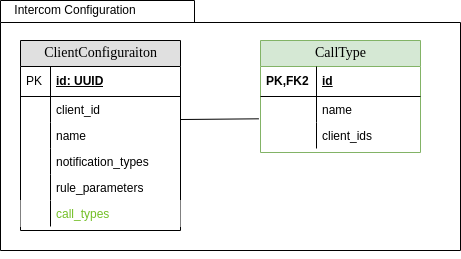
\includegraphics[width=\textwidth]{/home/joshua/FHNW/dev/IP6/IP6_Bachelorarbeit_Bericht_Cloudbasiertes_Praxisrufsystem/src/graphics/diagramms/erd_intercom_v02.drawio}}
        \caption{ERD Ausschnitt - Konfiguration Gegensprechanlage}
    \end{minipage}
\end{figure}

Das Admin UI wird mit Ansichten erweitert, über welche CallTypes erstellt, angezeigt, bearbeitet und gelöscht werden können.
Gleichzeitig wird der Cloudservice um Rest Endpunkte für das Lesen, Erstellen, Aktualisieren und Löschen von CallTypes erweitert.
Die Ansichten für ClientConfigurations im Admin UI werden so erweitert, dass CallTypes darauf angezeigt, hinzugefügt und entfernt werden können.
Die API des Cloudservice wird erweitert, um die erweiterte Konfiguration verwalten zu können.

\clearpage

\subsubsection{Signaling Instanz}

Mit WebRTC werden Peer-To-Peer Verbindungen aufgebaut~\cite{webrtc}.
Damit diese Verbindungen aufgebaut werden können, müssen die beteiligten Geräte Signalmeldungen austauschen können.
Dazu ist eine Instanz notwendig, welche Signale zwischen den Endgeräten vermitteln kann.
Diese Signaling Instanz wird als Teil des Cloudservice implementiert.

Der Cloudservice wird um ein neues Modul ''Signaling'' erweitert.
Dieses soll den Austausch von Signalen zwischen Clients ermöglichen.
Gleich wie das Modul für Sprachsynthese wird es unabhängig von den anderen Domänenmodulen im Cloudservice implementiert.
Das Modul Signaling muss dabei zwei Aufgaben übernehmen.
Erstens muss es Mobile Clients die Möglichkeit bieten, sich für Sprachverbindungen zu registrieren.
Zu diesem Zweck müssen Mobile Clients eine Verbindung mit der Signaling Instanz herstellen und trennen können.
Zweitens muss es Signalmeldungen empfangen und an die relevanten Empfänger zustellen können.
Kann eine Signalmeldung nicht zugestellt werden, muss es den betroffenen Empfänger über das verpasste Signal informieren.

Für diese Funktionen wird das Interface ClientConnector definiert.
Dieses definiert die Methoden afterConnectionEstablished und afterConnectionClosed.
Die beiden Methoden werden aufgerufen, wenn eine Verbindung geöffnet bzw.\ geschlossen wurde.
Die Implementierung dieses Interfaces ist dafür verantwortlich verfügbare Verbindungen zu verwalten.
Weiter definiert das Interface die Methode handleSignal.
Diese muss verwendet werden, um ein Signal entgegenzunehmen und an relevante Empfänger weiterzuleiten.

\begin{figure}[h]
    \centering
    \begin{minipage}[b]{1\textwidth}
        \fbox{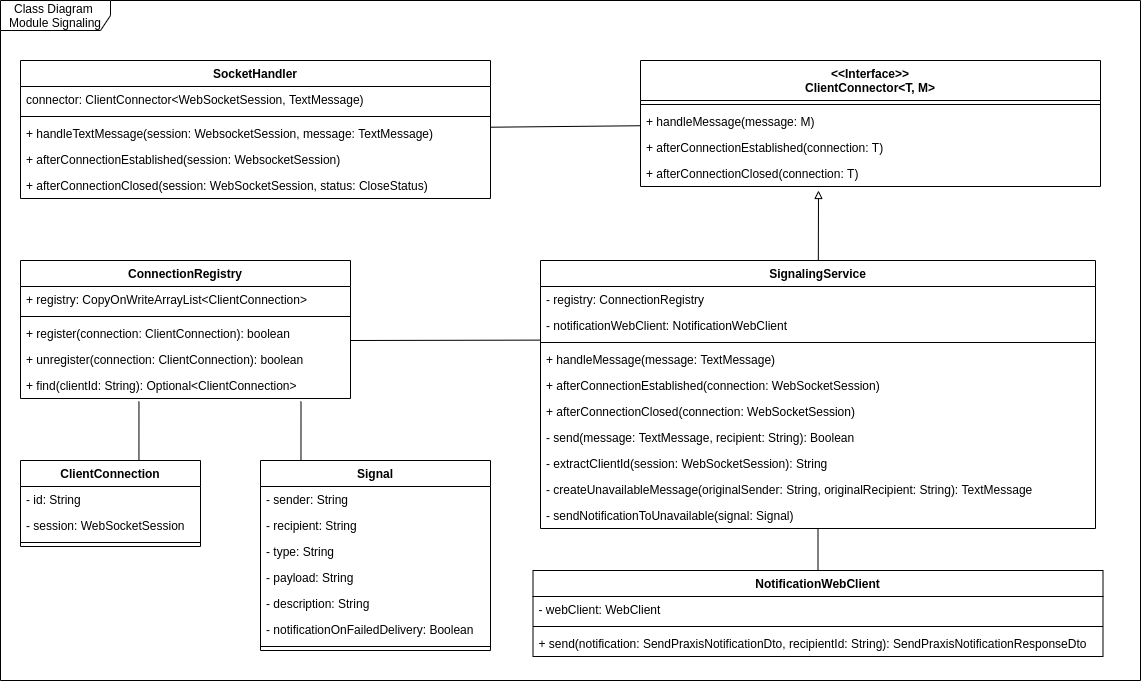
\includegraphics[width=\textwidth]{/home/joshua/FHNW/dev/IP6/IP6_Bachelorarbeit_Bericht_Cloudbasiertes_Praxisrufsystem/src/graphics/diagramms/Class_Intercom_Full_V01}}
        \caption{Klassendiagramm - Modul Signaling}
    \end{minipage}
\end{figure}

Für die Verwaltung von Verbindungen wird die Komponente ConnectionRegistry implementiert.
Diese führt eine Liste bekannter Verbindungen und bietet Methoden um Verbindungen zu registrieren und wieder entfernen.
Sie bietet weiter eine Methode, um zu überprüfen, ob eine bestimmte Verbindung bekannt ist.
Bekannte Verbindungen werden mit der Klasse ClientConnection abgebildet.
Ein ClientConnection beinhaltet immer einen Identifikator und das technische Verbindungsobjekt.
So können Verbindungen in der ClientConnection immer über einen eindeutigen Identifikator registriert und gefunden werden.

Die Klasse SignalingService implementiert das ClientConnector Interface.
Sie verwendet die Klasse ConnectionRegistry, um eine Liste von verfügbaren Verbindungen zu führen.
Über die Methoden onConnectionEstablished werden neue Verbindungen in der ConnectionRegistry registriert.
Mit der Methode onConnectionClosed werden geschlossene Verbindungen wieder entfernt.

Für das Zustellen von Signalen über bekannte Verbindungen wird die Methode handleSignal implementiert.
Jedes Signal beinhaltet die Identifikation seines Empfängers.
Beim Empfang eines Signals wird kontrolliert, ob die ConnectionRegistry eine Verbindung für die Identifikation des Empfängers enthält.
Ist dies der Fall, wird das Signal über diese Verbindung an den Empfänger übermittelt.
Wenn dies nicht der Fall ist oder wenn das Senden des Signals fehlschlägt, ist der Empfänger nicht erreichbar.
Nicht erreichbare Empfänger werden mit Benachrichtigungen über verpasste Signale informiert.
Dazu wird eine Benachrichtigung über die API des Moduls Notification versendet.

Die Schnittstelle der Signaling Instanz im Cloudservice wird mit Websockets umgesetzt.
Dazu wird die Bibliothek Spring-Boot-Starter-Websocket verwendet.
Es wird ein WebsocketHandler implementiert, welcher unter dem Pfad ''$<$serverUrl$>$/signaling'' erreichbar ist.
Etablierte Verbindungen müssen eindeutig einem Client zugeordnet werden können.
Diese Identifikation wird als Query Parameter bei Verbindungsaufbau mitgegeben.
Der WebsocketHandler definiert Methoden die beim Öffnen und Schliessen von Verbindungen sowie beim Empfang von Signalen aufgerufen werden.
Die Verarbeitung dieser Signale und Verbindungen wird an den SignalingService delegiert.

\subsubsection{Sicherheit für Signaling}

Der Zugriff auf die Signaling Instanz und die darüber ausgetauschten Signale darf nur für Berechtigte möglich sein.
Um dies sicherzustellen, wird der Verbindungsaufbau nur erlaubt, wenn die Anfrage dazu authentisiert ist.
Für die Authentisierung wird derselbe Mechanismus wie für Http-Anfragen der Cloudservice-API verwendet.
Durch die Konfiguration des Cloudservices wird die Authentifizierung aller Http Requests überprüft.
Mit dieser Prüfung wird sichergestellt, dass gültige Authentifizierungsdaten im Header der Anfrage vorhanden sind.
Ist dies nicht der Fall, wird eine entsprechende Fehlermeldung zurückgegeben.
Bei der Prüfung von Http-Anfragen durch den Cloudservice werden weiter die Rollen, welche dem Aufrufer zugeteilt sind ausgelesen.

Diese Prüfung der Authentifizierung wird auch für die Http-Anfragen, welche zum Aufbau einer Websocketverbindung nötig sind ausgeführt.
Beinhaltet eine Anfrage zum Aufbau einer Websocketverbindung keine gültige Authentifizierung, wird eine Fehlermeldung zurückgegeben.
Der Aufbau der Websocketverbindung wird abgebrochen.

Die Prüfung der ausgelesenen Rollen wird mit der Klasse HttpSessionHandshakeInterceptor implementiert.
Diese wird, nachdem eine Anfrage zum Aufbau einer Websocketverbindung eingegangen ist, aufgerufen.
Der HttpSessionHandshakeInterceptor erlaubt es die Anfrage zum Verbindungsaufbau auszulesen.
Dies erlaubt es hier zu verifizieren, dass der Request authentifiziert wurde und nur die zugeteilten Rollen zu überprüfen.
Praxisruf kennt die zwei Rollen ''ADMIN'' und ''USER''.
Beide Rollen sind berechtigt, dass Rufsystem über den Mobile Client zu verwenden und dürfen damit Signalmeldungen austauschen.
Hat der Aufrufer keine dieser Rollen, wird der Verbindungsaufbau abgebrochen.

Für Websocketverbindungen wird ausschliesslich das Protokoll Secure WebSockets (WSS) verwendet.
Die Http-Anfragen für den Verbindungsaufbau werden ausschliesslich über Https versendet.
Der Verbindungsaufbau und Austausch von Signalmeldungen über das Signaling Modul sind damit verschlüsselt.

\clearpage

\subsubsection{Anmeldung und Registrierung}

Dieses Kapitel beschreibt, welche Anmelde- und Registrierungsprozesse im Mobile Client benötigt werden.

Anmeldung und Registrierung für Benachrichtigungen funktionieren mit dem neuen Mobile Client nach demselben Ablauf wie im Vorgängerprojekt.
Die Registrierung für Sprachverbindungen beim Signaling Modul des Cloudservice wird mit diesem Projekt hinzugefügt.
Der gesamte Ablauf von Anmeldung und Registrierung wird in Abbildung 7.16 dargestellt.
Praxismitarbeitende öffnen die Applikation und geben ihr Benutzername und Passwort ein.
Der Mobile Client verwendet diese, um sich über Basic Authentication beim Cloudservice anzumelden.
Als Antwort auf die Anmeldung gibt der Cloudservice ein Json Web Token (JWT) zurück.
Dieses wird lokal auf dem Gerät gespeichert und für alle weiteren Anfragen an den Cloudservice verwendet.
Nachdem die Anmeldung erfolgt ist, wird eine Liste der verfügbaren Konfigurationen geladen.
Der Benutzer wählt die gewünschte Konfiguration aus und bestätigt.

\begin{figure}[h]
    \centering
    \begin{minipage}[b]{0.9\textwidth}
        \fbox{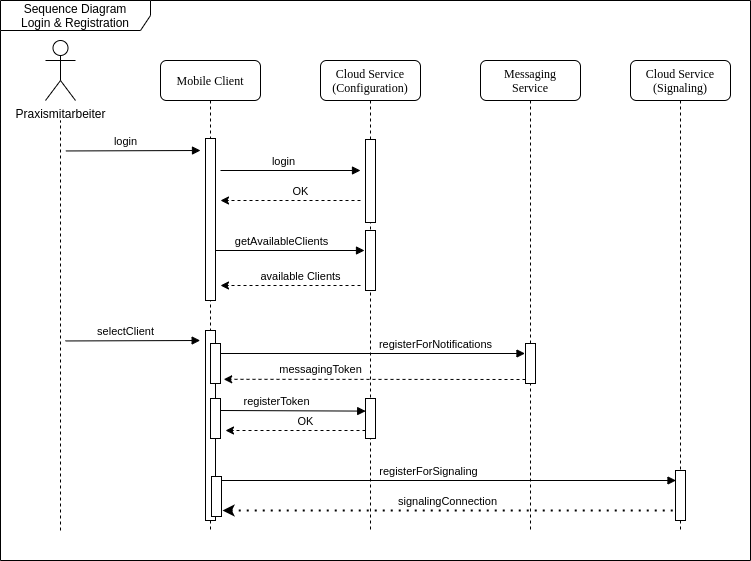
\includegraphics[width=\textwidth]{/home/joshua/FHNW/dev/IP6/IP6_Bachelorarbeit_Bericht_Cloudbasiertes_Praxisrufsystem/src/graphics/diagramms/Sequence_Registration}}
        \caption{Sequenzdiagramm - Anmeldung und Registrierung im Mobile Client}
    \end{minipage}
\end{figure}

Danach wird diese Konfiguration geladen und die Hauptansicht angezeigt.
Die geladene Konfiguration beinhaltet alle Informationen die nötig sind um Buttons für Benachrichtigungen und Sprachverbindungen anzuzeigen.
Im Hintergrund muss sich der Mobile Client nun für Benachrichtigungen und Sprachverbindungen registrieren.
Für Benachrichtigungen registriert er sich zuerst bei Firebase Cloud Messaging.
Er erhält ein Token, welches den Client beim Messaging Service identifiziert.
Dieses Token sendet der Mobile Client zusammen mit der gewählten Konfiguration an den Cloudservice.
Dieser persistiert die Registrierung und kann sie verwenden, um Benachrichtigungen an diesen Client zuzustellen.
Für Sprachverbindungen muss zudem eine Verbindung zum Signaling Modul des Cloudservices aufgebaut werden.
Dazu wird wie in Kapitel 7.4.6 beschrieben eine Websocketverbindung geöffnet.

\clearpage

\subsubsection{Signalmeldungen}

Dieses Kapitel beschreibt die Signalmeldungen, welche in Praxisruf verwendet werden.
Dabei wird beschrieben wie diese aufgebaut sind und welchen Rolle sie im System erfüllen.
Abbildung 7.17 zeigt, wie Signalmeldungen im Mobile Client modelliert werden.

\begin{figure}[h]
    \centering
    \begin{minipage}[b]{0.5\textwidth}
        \fbox{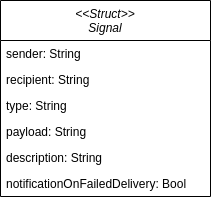
\includegraphics[width=\textwidth]{graphics/diagramms/Class_Signal}}
        \caption{Klassendiagramm - Signal}
    \end{minipage}
\end{figure}

Alle Signalmeldungen beinhalten Identifikation von Sender und Empfänger.
Diese werden von der Signaling Instanz verwendet, um die Signale korrekt weiterzuleiten.
Die Werte Type, Payload und Description werden im Mobile Client verwendet, um das Signal korrekt zu verarbeiten und Verbindungen aufzubauen.
Das Flag notificationOnFailedDelivery wird im Cloudservice ausgewertet.
Wenn ein Signal nicht zugestellt werden kann und dieses Flag aktiviert ist, wird der Empfänger mit einer Benachrichtigung darüber informiert.
Dazu wird die API des Notification Moduls des Cloudservices verwendet.

Praxisruf verwendet sechs Typen von Signalmeldungen.
Folgende Übersicht beschreibt pro Typ welche Daten ein Signal beinhaltet und welche Rolle es erfüllt.
\\
\begin{tabbing}
    Left \= Middle \= Right \= Right \kill
    Offer
    \> \> \> Wird vom Initiator der Sprachverbindung an die Empfänger gesendet. Ein Offer
    \\\> \> \> beinhaltet die SDP Informationen des Initiators und initiiert eine Verbindung. \\ \\

    Answer
    \> \> \> Wird vom Empfänger eines Offers an den Initiator der Sprachverbindung gesendet.
    \\\> \> \> Es beinhaltet SDP Informationen des Empfängers und bestätigt eine Verbindung. \\ \\

    Ice Candidate
    \> \> \> Beinhaltet Informationen eines ICE Candidates, die für den Verbindungsaufbau ver-
    \\ \> \> \> wendet werden. Nach Verarbeitung von Offer und Answer tauschen Initiator und
    \\ \> \> \> Empfänger solange Ice Candidate Signale aus, bis sie sich auf einen Kandidaten
    \\ \> \> \> geeinigt haben. Dieser wird verwendet, um die Verbindung aufzubauen.
    \\ \> \> \> \\

    End
    \> \> \> Wird versendet, nachdem die Verbindung durch tippen des Auflegen-Button in der
    \\ \> \> \> Applikation beendet wurde. Empfang dieses Signal führt dazu, dass offene Sprach-
    \\ \> \> \> verbindungen zum Sender dieses Signals beim Empfänger beendet werden.\\ \\

    Unavailable
    \> \> \> Wenn der Signalingserver ein Signal nicht zustellen kann, wird ein Unavailable-
    \\ \> \> \> Signal zurück an den Sender gesendet. Der Sender ist so informiert, dass die Ver-
    \\ \> \> \> bindung zum Gesprächspartner nicht aufgebaut wurde. \\ \\

    Decline
    \> \> \> Wird ein Offer empfangen während die Gegensprechanlage in den lokalen Einstel-
    \\ \> \> \> lungen deaktiviert ist oder bereits in Anruf aktiv ist, sendet der Mobile Client ein
    \\ \> \> \> Decline Signal zurück. Der Sender ist so informiert, dass die Verbindung zum Ge-
    \\ \> \> \> sprächspartner abgelehnt wurde.
\end{tabbing}

\clearpage

\subsubsection{Verbindungsaufbau}

Praxismitarbeitende können Sprachverbindungen zu anderen Clients aufbauen indem sie auf den entsprechenden Button in der Praxisruf App tippen.
Zum Zeitpunkt an dem der Button getippt wird, weiss der Mobile Client noch nicht, zu welchen Clients diese Verbindung aufgebaut werden soll.
Als Erstes muss deshalb beim Cloudservice angefragt werden, zu welchen Clients eine Sprachverbindung aufgebaut werden soll.
Der Cloudservice bietet dazu einen Endpoint an, über den der vollständige CallType des verwendeten Buttons geladen werden kann.
Nachdem diese Informationen geladen sind, können Sprachverbindungen zu allen Empfängern aufgebaut werden.
Dazu müssen Offer, Answer und Ice Candidate Signale ausgetauscht werden.
Der auslösende Client initialisiert die Peer-to-Peer Verbindung auf seiner Seite und sendet für jeden Gesprächspartner ein Offer.
Der Cloudservice findet die Verbindung der jeweiligen Empfänger und leitet die Signale über deren Verbindung weiter.

Nach Eingang des Offer-Signals wird die Verbindung auf Empfängerseite initialisiert und eine Answer zurück an den Initiator gesendet.
Diese wird gleich wie das Offer-Signal über die Signaling Instanz zugestellt.
Der Initiator empfängt die Antwort Signale und ergänzt die notwendigen Verbindungsinformationen.
Abbildung 7.18 visualisiert diesen Ablauf.

\begin{figure}[h]
    \centering
    \begin{minipage}[b]{0.9\textwidth}
        \fbox{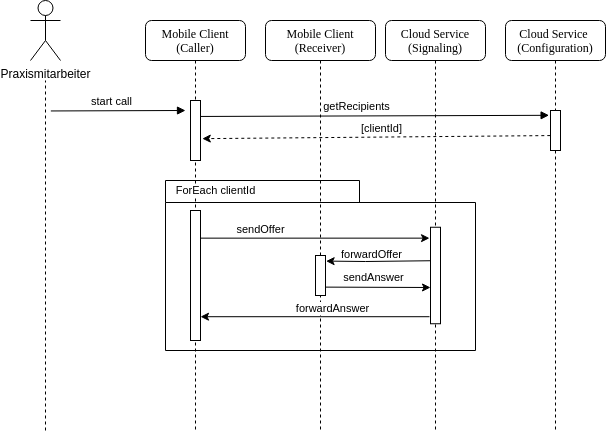
\includegraphics[width=\textwidth]{graphics/diagramms/Sequence_Intercom_Broking_V02}}
        \caption{Sequenzdiagramm - Verbindungsaufbau mit Offer und Answer Signalen}
    \end{minipage}
\end{figure}

Nachdem die Offer und Answer Meldungen ausgetauscht sind, müssen Ice Candidate Meldungen ausgetauscht werden.
Der Austausch von Ice Candidate Meldungen wird so lange wiederholt, bis sich beide Seiten einer Verbindung auf Verbindungsdetails geinigt haben.
Sobald dieser Austausch beendet ist, besteht die Verbindung und es können Sprachdaten ausgetauscht werden.

\clearpage

\subsubsection{Anbindung Mobile Client an Singaling Instanz}

Dieses Kapitel beschreibt, wie Websockeverbindungen zum Austausch von Signalmeldungen in den nativen Mobile Client integriert werden.

In Kapitel 7.2 wird die Klasse PraxisrufApi beschrieben.
Diese implementiert die Anbindung and die Http-API des Cloudservice.
Um Signalmeldungen über die Signaling Instanz des Cloudservice auszutauschen, müssen Websockets verwendet werden.
Damit die Anbindung an alle Schnittstellen des Cloudservice einheitlich bleibt, wird PraxisrufApi erweitert, um auch Websocketverbindungen zu unterstützen.
Dies beinhaltet den Auf- und Abbau von Verbindungen, sowie das Senden und Empfangen von Meldungen über diese Verbindung.
Weiter müssen Verhalten beim Empfang von Fehlermeldungen und dem unerwarteten Schliessen der Verbindung definiert werden.

Der Austausch von Signalmeldungen ist der einzige Anwendungsfall für Websockets in Praxisruf.
Deshalb wird auf eine generische Integration von Websockets verzichtet.
Zur Erweiterung von PraxisrufApi werden die Extension PraxisrufApi+Signaling und das Protokoll PraxisrufApiSignalingDelegate definiert.
Diese setzen die Anbindung von Websockets für den Austausch von Signalmeldungen um.

\begin{figure}[h]
    \centering
    \begin{minipage}[b]{0.6\textwidth}
        \fbox{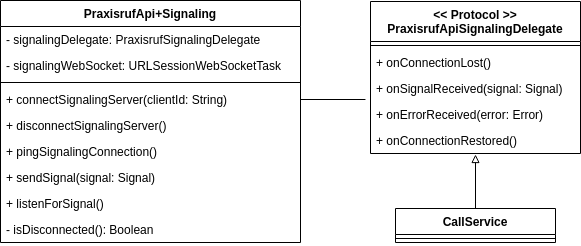
\includegraphics[width=\textwidth]{graphics/diagramms/Class_Mobile_Client_Signaling_Connection}}
        \caption{Klassendiagramm - Signaling Schnittstelle in Mobile Client}
    \end{minipage}
\end{figure}

Die Extension PraxisrufApi+Signaling ist für die Verbindung zu der Signaling Instanz verantwortlich.
Für die Integration dieser Extension in den Rest der Applikation wird das Protokoll PraxisrufApiSignalingDelegate definiert.
Zum Aufbau der Verbindung zu der Signaling Instanz wird die Methode connectSignalingServer definiert.
Die Identifikation des Clients wird bei dieser Abfrage als Parameter mitgegeben.
So kann die Verbindung von der Signaling Instanz eindeutig einem Client zugeordnet werden.
Nachdem die Verbindung geöffnet ist, können Signale empfangen und verarbeitet werden.
Dies wird durch die Methode listenForSignal initialisiert.
Darin wird der Websocketverbindung signalisiert, dass der Client bereit ist die nächste Meldung zu empfangen.
Sobald eine Meldung empfangen wird, wird diese über den PraxisrufApiSignalingDelegate verarbeitet.
Wurde eine gültige Signalmeldung empfangen, wird diese über die Methode onSignalReceived verarbeitet.
Wurde hingegen eine ungültige Signalmeldung oder eine Fehlermeldung empfangen wird die Methode onErrorReceived aufgerufen.
Im Fehlerfall wird zudem überprüft, ob die Verbindung noch offen verwendbar ist.
Sollte die Verbindung nicht mehr verwendbar sein, wird die Methode onConnectionLost des Delegates aufgerufen.
Dadurch wird versucht, die Verbindung erneut aufzubauen.
Ist dies nicht möglich, wird eine Fehlermeldung angezeigt. 

PraxisrufApi+Signaling definiert weiter Methoden um Signal- und Pingmeldungen zu versenden.
Pingmeldungen werden in Regelmässigen Abständen gesendet um sicherzustellen, dass die Verbindung zu der Signaling Instanz geöffnet bleibt.
Vor dem Senden jeder Meldung wird geprüft, ob die Verbindung zur Signaling Instanz verwendbar ist.
Ist dies nicht der Fall, wird die Methode onConnectionLost des Delegates aufgerufen und anschliessend versucht die Meldung zu versenden.
Schlägt das Senden fehl, wird die Methode onErrorReceived auf dem Delegate aufgerufen.

Die Methoden des Protokolls CallClientDelegate werden durch die Klasse CallService implementiert.
Der CallService vermittelt Anfragen zwischen Signaling Instanz, Benutzeroberfläche und Peer-To-Peer Verbindungen im Mobile Client.
Er ist dafür verantwortlich Signale an die Peer-To-Peer Verbindung weiterzuleiten, geschlossene Verbindungen wieder zu öffnen und Fehlermeldungen anzuzeigen.
Empfangene Signalmeldungen werden über die Methode onSignalReceived an die Komponente CallClient übergeben (Siehe Kapitel 7.4.9).
Die Methoden onConnectionLost und onErrorReceived werden verwendet, um Fehlermeldungen anzuzeigen und geschlossene Verbindungen erneut zu öffnen.
Nachdem die Verbindung zur Signaling Instanz verloren gegangen ist, wird bis zu zehnmal versucht, die Verbindung erneut zu öffnen.
Wenn die Verbindung dadurch nicht repariert werden kann, wird sie geschlossen und dem Benutzer eine Fehlermeldung angezeigt.

\subsubsection{Verbindungsverwaltung}

Dieses Kapitel beschreibt, wie im Mobile Client sichergestellt wird, dass die Verbindung zu der Signaling Instanz langfristig zur Verfügung steht.
Abbildung 7.20 gibt einen Überblick, über die Abläufe dazu umgesetzt werden.
Dieser Ablauf ist mit den Komponenten CallService und PraxisrufApi+Signaling die, in Kapitel 7.4.7 beschrieben sind, implementiert.

\begin{figure}[h]
    \centering
    \begin{minipage}[b]{1\textwidth}
        \fbox{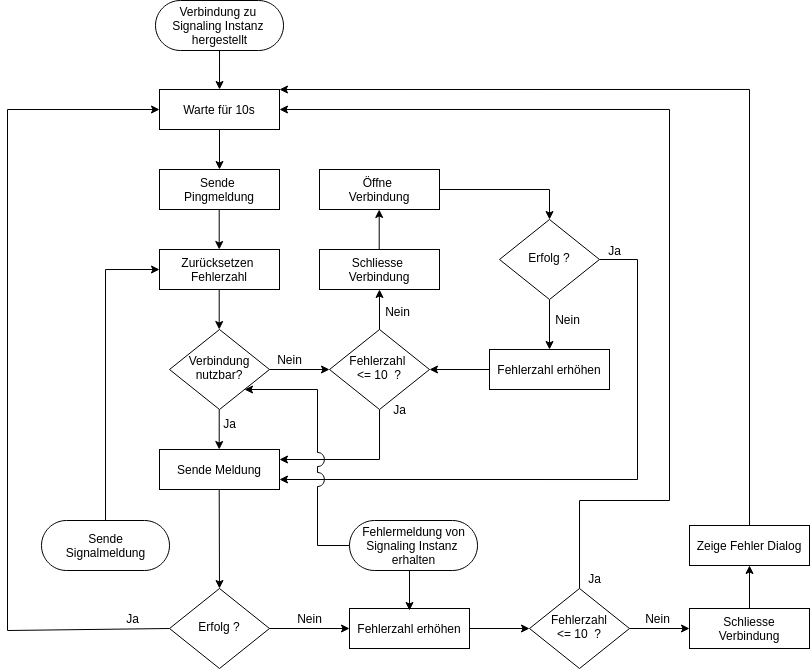
\includegraphics[width=\textwidth]{graphics/diagramms/flow_connection}}
        \caption{Flowchart - Verbindungsverwaltung}
    \end{minipage}
\end{figure}

Um festzustellen, ob die eine getrennte Verbindung repariert werden kann, wird im CallService ein Fehlerzähler geführt.
Dieser wird beim Start der Applikation mit null initialisiert und bei jedem Verbindungsfehler um eins inkrementiert.
Ein Verbindungsfehler tritt auf, wenn eine Fehlermeldung über die Signaling Verbindung empfangen wird und wenn das Senden einer Meldung oder das Wiederherstellen der Verbindung fehlschlägt.

Die Verbindung zur Signaling Instanz wird hergestellt, sobald die Applikation gestartet wird.
Nachdem die Verbindung hergestellt wurde, werden im Abstand von zehn Sekunden Pingmeldungen über die Verbindung gesendet.
Dadurch wird sichergestellt, dass die Verbindung geöffnet bleibt.
Vor dem Versenden jeder Meldung wird der Fehlerzähler zurückgesetzt und es wird überprüft, ob die Verbindung verwendet werden kann.
Ist die Verbindung fehlerhaft, werden bis zu zehn Versuche unternommen, sie wiederherzustellen.
Anschliessend wird versucht, die Meldung zu versenden.
Wenn die Meldung erfolgreich versendet wurde, wird der Fehlerzähler zurückgesetzt und zehn Sekunden gewartet, bis die nächste Pingmeldung versendet wird.
Andernfalls wird die Fehlerzahl um eins erhöht.
Ist die Fehlerzahl danach grösser als zehn, wird die Verbindung getrennt.
In der Benutzeroberfläche wird ein Fehlerdialog angezeigt.
Die Verbindung bleibt geschlossen bis die nächste Meldung versendet wird.
Dies der Fall, wenn das Interval für die nächste Pingmeldung abgelaufen ist oder wenn ein Anruf über die Benutzeroberfläche gestartet wird.

Bei Start eines Anrufes aus der Benutzeroberfläche werden dieselben Prüfungen, wie vor dem Versenden von Pingmeldungen ausgeführt.
So werden geschlossene Verbindungen zur Signaling Instanz frühzeitig repariert.
Weiter wird nach Empfang jedes Fehlers über die Signaling Verbindung geprüft, ob diese noch offen ist.
Ist dies nicht der Fall, werden auch hier bis zu zehn Versuche unternommen, die Verbindung wiederherzustellen.

Dieser Ablauf stellt sicher, dass die Verbindung zu der Signaling Instanz geöffnet bleibt und wenn nötig repariert wird.
Wenn möglich, geschieht dies direkt nach Verbindungsverlust.
Andernfalls werden Praxismitarbeitende informiert, dass die Verbindung nicht hergestellt werden konnte.
Im Hintergrund wird in dieser Situation regelmässig versucht, die Verbindung zu reparieren.
Die Bedienelemente für die Gegensprechanlage bleiben während dieser Zeit aktiviert und können weiter verwendet werden.
Wenn Praxismitarbeitende einen Anruf starten und die Verbindung immer noch getrennt ist, wird die sie frühzeitig wiederhergestellt.
Ist dies erfolgreich, wird der Anruf gestartet.
Andernfalls wird erneut ein Fehlerdialog angezeigt.

\clearpage

\subsubsection{Sprachverbindungen im Mobile Client}

Dieses Kapitel beschreibt wie WebRTC-Komponenten in den Mobile Client integriert werden, um Sprachverbindungen zu ermöglichen.

Für die Integration der WebRTC-Komponenten wird eine Klasse CallClient und ein Protokoll CallClientDelegate erstellt.
Der CallClient verwaltet Sprachverbindungen, während der Delegate zur Integration mit der restlichen Applikation dient.
Abbildung 7.21 zeigt das Klassendiagramm beider Komponenten.
Die Methoden des CallClientDelegate-Protokolls werden von der Klasse CallService implementiert.
Da diese Klasse auch das Protokoll SignalingDelegate implementiert, kann sie verwendet werden um Signalmeldungen zwischen CallClient und PraxusrufApi+Signaling zu vermitteln.

\begin{figure}[h]
    \centering
    \begin{minipage}[b]{0.6\textwidth}
        \fbox{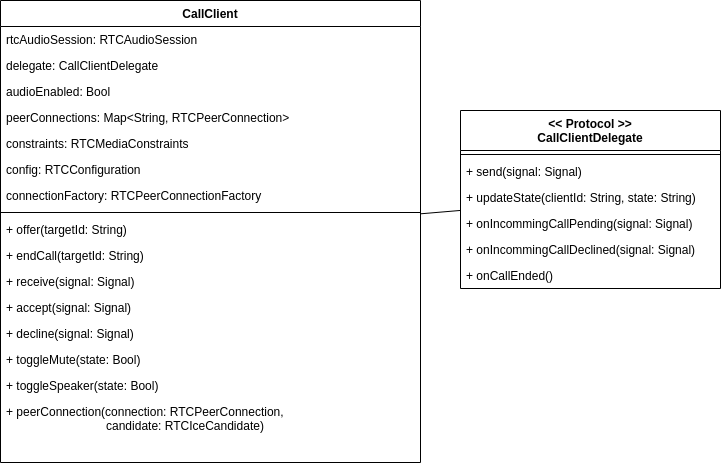
\includegraphics[width=\textwidth]{graphics/diagramms/Class_Mobile_Client_Signal_Processing}}
        \caption{Klassendiagramm - CallClient und CallClientDelegate}
    \end{minipage}
\end{figure}

Für den Aufbau von ausgehenden Verbindungen wird eine RTCPeerConnection im CallClient des Senders initialisiert.
Es werden die SDP Informationen für Beschreibung der Verbindung erstellt und mit einem Offer-Signal an den Empfänger gesendet.
Dieses Offer-Signal wird über den CallClientDelegate versendet, welcher das Signal an die Signaling Instanz zustellt.

Für den Aufbau von eingehenden Verbindungen wird das Offer-Signal über die Methode receive empfangen.
Dabei wird die Verbindung nicht direkt initialisiert.
Stattdessen wird das Signal zwischengespeichert und die Methode onIncommingCallPending des Delegates aufgerufen.
Die Implementation des CallClientDelegate navigiert darauf zu der Ansicht für aktive Anrufe und meldet dem CallClient über die Methode acceptPending, dass die Verbindung initialisiert werden soll.
Der CallClient initialisiert darauf eine RTCPeerConnection und sender ein Answer Signal über die send Methode.

Answer-Signale werden ebenfalls über die receive Methode im CallClient empfangen.
Beim Empfang einer Answer werden die SDP Informationen auf der lokalen RTCPeerConnection ergänzt.

Neben dem Austausch von Offer- und Answer-Signalen müssen Ice Candidate Signale ausgetauscht werden können.
Sobald ein Ice Candidate zur Verfügung steht, erstellt der CallClient ein entsprechendes Signal und sendet es an den Empfänger.
Damit dies möglich ist, muss der CallClient über verfügbare Ice Candidates informiert werden.
Die WebRTC Bibliothek bietet dazu das Protokoll RTCPeerConnectionDelegate.
Dieses kann auf der RTCPeerConnection registriert werden und wird aufgerufen, sobald ein neuer Ice Candidate verfügbar ist.
Der CallClient implementiert dieses Protokoll und registriert sich auf allen RTCPeerConnections als Delegate.

Sprachverbindungen müssen über die Benutzeroberfläche verwaltet werden können.
Der CallClient bietet deshalb Methoden an, um eine Verbindung zu starten und beenden.
Weiter bietet er die Möglichkeit Mikrofon und Lautsprecher für geöffnete Verbindungen stummzuschalten.
Bei eingehenden Verbindungen, dem Beenden von Anrufen und Veränderungen am Status einer Verbindung, muss die Benutzeroberfläche informiert werden.
Der CallClientDelegate definiert dazu Methoden über welche der CallClient diese Informationen weitergeben kann.

\subsubsection{Signalverarbeitung im Mobile Client}

Peer-To-Peer Sprachverbindungen werden über die Komponenten CalService, CallClient und PraxisrufApi+Signaling in den Mobile Client integriert.
Dieses Kapitel beschreibt den Kommunikationsablauf zwischen diesen Komponenten anhand des Austauschs von Offer- und Answer-Signalen.

\begin{figure}[h]
    \centering
    \begin{minipage}[b]{0.85\textwidth}
        \fbox{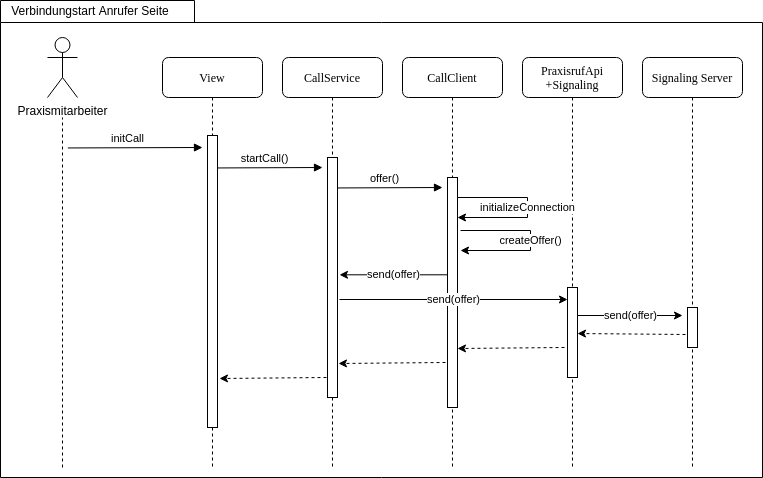
\includegraphics[width=\textwidth]{/home/joshua/FHNW/dev/IP6/IP6_Bachelorarbeit_Bericht_Cloudbasiertes_Praxisrufsystem/src/graphics/diagramms/Sequence_MobileClient_Caller_Signaling.drawio}}
        \caption{Sequenzdiagramm - Initialisierung Sprachverbindung auf Senderseite }
    \end{minipage}
\end{figure}


Die Klassen CallClient und PraxisrufApi+Signaling definieren je ein Delegate-Protokoll.
Diese Protokolle definieren die Funktionen, über welche die Komponenten Informationen weitergeben können.
Die Klasse CallService implementiert beide Delegate-Protokolle.
Er erstellt Instanzen von CallClient und PraxisrufApi+Signaling und registriert sich anschliessend bei beiden als Delegate.
Der CallService selbst wird in den View Komponenten der Applikation verwendet.
Er nimmt Benutzereingaben entgegen und delegiert die entsprechende Funktionalität an den CallClient und PraxisrufApi+Signaling.
Er nimmt ausserdem Informationen von CallClient und PraxisrufApi+Signaling entgegen und stellt Anzeigeinformationen für die Benutzeroberfläche zur Verfügung.

Abbildung 7.22 zeigt die Kommunikation zwischen den beteiligten Komponenten bei der Initialisierung einer Sprachverbindung auf Empfängerseite.
Dabei wird der Ablauf von Benutzerinteraktion des Senders bis zum Senden des Offer-Signals dargestellt.
Sobald Praxismitarbeitende einen Anruf startet, wird die View für aktive Anrufe geladen.
Diese initialisiert den Anruf über den CallService.
Der CallService ruft dazu als Erstes den CallClient auf.
Der CallClient initialisiert die lokalen Verbindungsinformationen und erstellt ein Signal, um den Empfänger zu informieren.
Dieses Signal gibt er an den CallService weiter.
Der CallService leitet das Signal an den PraxisrufApi+Signaling weiter, welcher das Versenden an den Cloudservice übernimmt.

\begin{figure}[h]
    \centering
    \begin{minipage}[b]{0.85\textwidth}
        \fbox{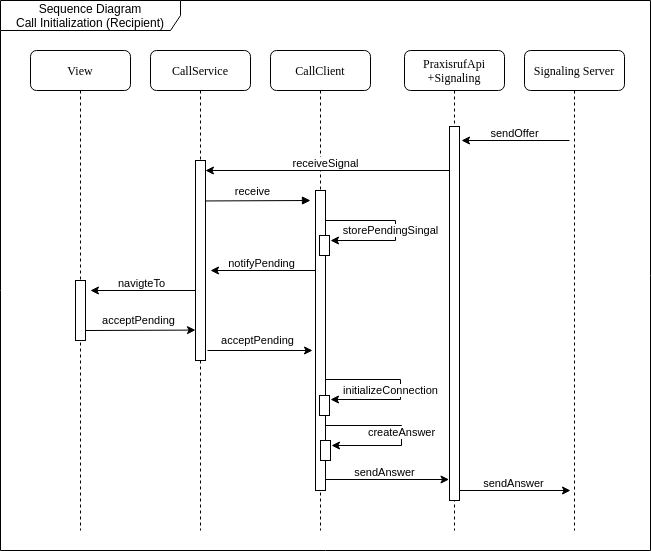
\includegraphics[width=\textwidth]{/home/joshua/FHNW/dev/IP6/IP6_Bachelorarbeit_Bericht_Cloudbasiertes_Praxisrufsystem/src/graphics/diagramms/Sequence_MobileClient_Receiver_Signaling.drawio.png}}
        \caption{Sequenzdiagramm - Initialisierung Sprachverbindung auf Empfängerseite }
    \end{minipage}
\end{figure}


Abbildung 7.23 zeigt den Ablauf bei Eingang eines Answer-Signals auf Empfängerseite.
Das versendete Signal wird über das Signaling Modul des Cloudservice an den Empfänger übermittelt.
Dieser empfängt das Signal über die Komponente PraxisrufApi+Signaling.
Diese gibt das Signal über die Methode onSignalReceived an den CallService weiter.
Der CallService aktiviert die Ansicht für aktive Anrufe und leitet das Signal an den CallClient weiter.
Der CallClient initialisiert die Peer-To-Peer Verbindung und erstellt ein Answer-Signal zur Bestätigung.
Dieses Signal wird wiederum über den CallService zum PraxisrufApi+Signaling weiter zum Cloudservice versendet.


\subsubsection{Netzwerkvoraussetzungen}

Praxisruf ist darauf ausgelegt innerhalb von Arztpraxen verwendet zu werden.
Dabei wird pro Zimmer ein Gerät installiert, welches als Endpunkt für das System dient~\cite{aufgabenstellung}.
Damit werden alle Endgeräte innerhalb derselben Praxis betrieben.
Dies erlaubt es, die Geräte über ein lokales Netzwerk zu verbinden.
Ist diese Voraussetzung gegeben, kann der Verbindungsaufbau vereinfacht werden.
Da die Geräte direkt im lokalen Netzwerk kommunizieren können, ist es nicht nötig, die Protokolle STUN oder TURN zu verwenden.
Damit wird es möglich auf den Betrieb eines ICE Servers zu verzichten.
Die Geräte können ICE Kandidaten für direkte Kommunikation im lokalen Netzwerk austauschen.

Die Integration von WebRTC in der iOS App wird unter der Voraussetzung umgesetzt, dass alle beteiligten Geräte im selben Netzwerk betrieben werden.
Dies vereinfacht den Aufbau von Verbindungen und erlaubt es, neben der Signaling Instanz keine weitere Infrastruktur betreiben zu müssen.
Sprachverbindungen mit Praxisruf sind deshalb nur möglich, wenn die beteiligten Geräte im selben lokalen Netzwerk betrieben werden.
Das Versenden und Empfangen von Benachrichtigungen funktioniert wie im Vorgängerprojekt auch ausserhalb des lokalen Netzwerkes.
Damit können auch für Empfänger, die nicht im lokalen Netzwerk sind, über verpasste Anrufe mit Benachrichtigungen informiert werden.

\clearpage

